%%%  Šablona práce od:
%%%  Copyright (C) 2012 Martin Rotter, <rotter.martinos@gmail.com>
%%%  Copyright (C) 2014 Jan Outrata, <jan.outrata@upol.cz>

%%  Pro získání PDF souboru dokumentu je třeba tento zdrojový text v
%%  LaTeXu přeložit (dvakrát) programem pdfLaTeX.

%%  V případě použití programu BibLaTeX pro tvorbu seznamu literatury
%%  je poté ještě třeba spustit program Biber s parametrem jméno
%%  souboru zdrojového textu bez přípony a následně opět (dvakrát)
%%  přeložit zdrojový text programem pdfLaTeX.

%%  Postup získání Postscriptového souboru je popsán v dokumentaci.

%%  Třída dokumentu implementující styl pro závěrečnou práci. Vybrané
%%  nepovinné parametry (ostatní v dokumentaci):

%%  'master' pro sazbu diplomové práce, jinak se sází bakalářská práce

%%  'program=kód' pro Váš studijní program/obor (specializaci), kódy
%%  pro diplomovou práci 'infoi' pro Informatiku (Obecná informatika),
%%  'infui' pro Informatiku (Umělá inteligence), 'ainfpst' pro
%%  Aplikovanou informatiku (Počítačové systémy a technologie), 'uinf'
%%  pro Učitelství informatiky pro střední školy, 'binf' pro
%%  Bioinformatiku, 'inf' pro Informatiku (bez specializací) a 'ainf'
%%  pro Aplikovanou informatiku (bez specializací), jinak je výchozí
%%  ainfvs pro Aplikovanou informatiku (Vývoj software), a pro
%%  bakalářskou práci 'infoi' pro Informatiku (Obecná informatika),
%%  'itp' pro Informační technologie v prezenční formě, 'itk' pro
%%  Informační technologie v kombinované formě, 'infv' pro Informatiku
%%  pro vzdělávání, 'binf' pro Bioinfomatiku, 'inf' pro Informatiku
%%  (bez specializací), 'ainfp' pro Aplikovanou informatiku (bez
%%  specializací) v prezenční formě, 'ainfk' pro Aplikovanou
%%  informatiku (bez specializací) v kombinované formě, jinak je
%%  výchozí infpvs pro Informatiku (Programování a vývoj software)

%%  'printversion' pro sazbu verze pro tisk (nebarevné logo a odkazy,
%%  odkazy s uvedením adresy za odkazem, ne odkazy do rejstříku),
%%  jinak verze pro prohlížeč

%%  'biblatex' pro zapnutí podpory pro sazbu bibliografie pomocí
%%  BibLaTeXu, jinak je výchozí sazba v prostředí thebibliography

%%  'language=jazyk' pro jazyk práce, jazyky english pro anglický,
%%  slovak pro slovenský, jinak je výchozí czech pro český

%%  'font=sans' pro bezpatkový font (Iwona Light), jinak je výchozí
%%  serif pro patkový (Latin Modern)

%%  'figures, tables, theorems a sourcecodes' pro sazbu seznamu
%%  obrázků, tabulek, vět a zdrojových kódů, jinak při =false se
%%  nesází (u theorems a sourcecodes výchozí)

\documentclass[
%  master,
%  program=ainfvs,
%  printversion,
  biblatex,
%  language=english,
%  font=sans,
  figures=true,
  tables=false,
%  theorems,
%  sourcecodes,
  glossaries,
  index
]{kidiplom}

%% Informace pro úvodní strany. V jazyku práce (pokud není v komentáři
%% uvedeno česky) a anglicky. Uveďte všechny, u kterých není v
%% komentáři uvedeno, že jsou volitelné. Při neuvedení se použijí
%% výchozí texty. Text pro jiný než nastavený jazyk práce (nepovinným
%% parametrem language makra \documentclass, výchozí český) se zadává
%% použitím makra s uvedením jazyka jako nepovinného parametru.

%% Název práce, česky a anglicky. Měl by se vysázet na jeden řádek.
\title{Multiplatformní aplikace pro správu osobních financí}
\title[english]{Cross-platform application for personal finance management}

%% Jméno autora práce. Makro nemá nepovinný parametr pro uvedení
%% jazyka.
\author{Vojtěch Netrh}

%% Jméno vedoucího práce (včetně titulů). Makro nemá nepovinný
%% parametr pro uvedení jazyka.
\supervisor{doc. RNDr. Jan Konečný, Ph.D.}

%% Volitelný rok odevzdání práce. Výchozí je aktuální (kalendářní)
%% rok. Makro nemá nepovinný parametr pro uvedení jazyka.
\yearofsubmit{2025}

%% Anotace práce, včetně anglické (obvykle překlad z jazyka
%% práce). Jeden odstavec!
\annotation{Ukázkový text závěrečné práce na Katedře informatiky
  Přírodovědecké fakulty Univerzity Palackého v Olomouci, který je
  zároveň dokumentací stylu pro text práce v \LaTeX{}u. Zdrojový text
  v \LaTeX{}u je doporučeno použít jako šablonu pro text skutečné
  závěrečné práce studenta.}

\annotation[english]{Sample text of thesis at the \kitextdepten,
  \kitextfacultyen, \kitextuniven{} and, at the same time,
  documentation of the \LaTeX{} style for the text. The source text in
  \LaTeX{} is recommended to be used as a template for real student's
  thesis text.}

%% Klíčová slova práce, včetně anglických. Oddělená středníkem.
\keywords{Flutter; Dart; multiplatformní; osobní finance}
\keywords[english]{Flutter; Dart; cross-platform; personal finance}

%% Volitelná specifikace příloh textu práce, i anglicky. Výchozí je
%% 'elektronická data v systému katedry informatiky / electronic data
%% in system of department of computer science'.
%\supplements{nejlepší software všech dob}
%\supplements[english]{the best software of all times}

%% Volitelné poděkování. Stručné! Výchozí je prázdné. Makro nemá
%% nepovinný parametr pro uvedení jazyka.
\thanks{Děkuji panu doc. RNDr. Janu Konečnému Ph. D. za cenné rady a podněty při tvorbě práce. Svým blízkým za podporu běheme celého bakalářského studia.}

%% Cesta k souboru s bibliografií pro její sazbu pomocí BibLaTeXu
%% (zvolenou nepovinným parametrem biblatex makra
%% \documentclass). Použijte pouze při této sazbě, ne při (výchozí)
%% sazbě v prostředí thebibliography.
\bibliography{bibliografie.bib}

%% Další dodatečné styly (balíky) potřebné pro sazbu vlastního textu
%% práce.
\usepackage{longtable}
\usepackage{svg}

\begin{document}
%% Sazba úvodních stran -- titulní, s bibliografickými údaji, s
%% anotací a klíčovými slovy, s poděkováním a prohlášením, s obsahem a
%% se seznamy obrázků, tabulek, vět a zdrojových kódů (pokud jejich
%% sazba není vypnutá).
\maketitle

%% Vlastní text závěrečné práce. Pro povinné závěry, před přílohami,
%% použijte prostředí kiconclusions. Povinná je i příloha s obsahem
%% elektronických dat.

%% -------------------------------------------------------------------

\newcommand{\BibLaTeX}{\textsc{Bib}\LaTeX}

% ----- tady začíná MNOU PSANÝ TEXT

\section{Úvod}
Peníze se vyskytují všude kolem nás a chceme-li nebo ne, hrají v našich životech podstatnou roli. Z hlediska osobního pohledu jednoho člověka je užitečné mít ve svých financích pořádek. Můžeme tak ušetřit peníze, případně je efektivněji využívat. V~neposlední řadě by měl člověk vědět, kolik peněz by potřeboval v~případě výpadku příjmů a jaká má být jeho \uv{železná rezerva}.

V dnešní době již většina lidí používá internetové bankovnictví, která dost často poskytuje alespoň základní statistiky o našem nakládání s financemi. Na druhou stranu lidé mívají účty u více bank a reporty o stavu financí nejsou dostatečně přizpůsobitelné.

Kromě toho, že peníze se podaří člověku ušetřit je vhodné s nimi potom dále nakládat. Můžeme je ihned utratit (což není dlouhodobě vhodná varianta), spořit si nebo dále investovat. Spořit si je možné na řadu věcí -- nové bydlení, automobil či vytvoření dostatečného objemu pěnez pro založení vlastního podnikání. Pro spoření existují dva základní způsoby jak peníze ukládat. Prvním z nich je mít je na běžném či spořícím účtu a jejich hodnota bude v čas pořád zhruba stejná. Druhým přístupem je aktivně investovat a snažit se pomocí nich vydělat další peníze.

\subsection{Požadavky}
Napsat něco jiného než minule, vhodný začátek podkapitoly.

\begin{itemize}
  \item \textbf{Jednoduchost více než komplexní funkce} -- snažit se implementovat dostatečný počet funkcí, avšak nezahltit uživatele příliš mnoha různými nastaveními, které mu přidají práci při volení parametrů. Pokud je pro uživatele pohodlné zapisovat transakce již v průběhu dne, aniž by měl pocit, že u aplikace tráví moc času, je to ideální scénář.
  \item \textbf{Mobilní telefony i počítače} -- obsáhnout zařízení na různé škále velikosti přináší dostupnost aplikace pro více uživatelů. Někdo rád evidenci financí dělá na denní bázi (obvykle pomocí mobilního telefonu), někdo naopak až měsíc zpětně. Na zpracování více dat najednou je jistě počítač s větším displejem vhodnější volbou.
  \item \textbf{Zahraniční měny} -- V dnešní době velká část lidí cestuje jak pracovně, tak i za dovolenou. Placení kartou v zahraničí bez nutnosti dopředu směnit peníze se stalo standardem. Jelikož každá banka používá jiný směnný kurz měny, měl by jít libovolně upravit, případně automaticky synchronizovat z internetu.
  \item \textbf{Export dat} -- uživatel by měl mít možnost exportovat data v běžně používaných formátech jako je CSV nebo JSON. Export považuji za důležitý z důvodu přenesení dat do jiného prostředí či aplikace.
\end{itemize}

\section{Přehled existujících řešení}
K danému tématu již existuje řada aplikací nabízejících nástroje pro správu financí. Každé řešení přistupuje k problému jiným způsobem. 

Nejblíže je z hlediska uživatele poskytnutí základních nástrojů přímo v bankovní aplikaci. Z mého pohledu je to nejméně vhodné řešení hned z několika důvodů:
\begin{itemize}
  \item obvykle má člověk účet u více bank (aplikace jedné z nich neposkytuje přehled o celkových financích),
  \item jen část (i když v dnešní době většinová) transakcí je prováděna pomocí platební karty,
  \item uživatel nemusí chtít mít všechny pohyby na účtu zahrnuty do celkové analýzy.
\end{itemize}

Aplikace třetích stran v tomto segmentu, nabízí různé možnosti. Mobilní aplikace bývají obvykle jednodušší a s přívětivějším uživatelským rozhraním. Zatímco desktopové aplikace mají uživatelské rozhraní spíše starší, avšak poskytují nepřebernou škálu funkcí.

\subsection{1Money}
Ještě na konci roku 2024 byla aplikace 1Money dostupná na obě mobilní platformy, o pár měsíců později už pouze na iOS. Z mnou vyzkoušených aplikací největší favorit pro denní užití. Aplikace mě zaujala svojí obrazovkou \textit{Categories}.  Středem obrazovky je prstencový graf zobrazující poměr utracených peněz podle kategorií a v jeho středu se ještě nachází dva údaje - stav příjmů a výdajů. Zbytek obrazovky pokrývají kolečka označující kategorie, po jejichž stisknutí je uživateli ihned umožněno přidat transakci s danou kategorií a aktuálním časovým razítkem. Velmi intuitivní a rychlé řešení pro každodenní použití. Umožňuje vytvořit více různých účtů, včetně účtů pro spoření. Z hlediska analýzy a grafů zde najdeme pouze dvě velmi omezené možnosti - již zmíněný prstencový graf kategorií a sloupcový graf znázornění transakcí v čase. Tuto aplikaci jsem si já osobně oblíbil nejvíce.

\begin{figure}
    \centering
    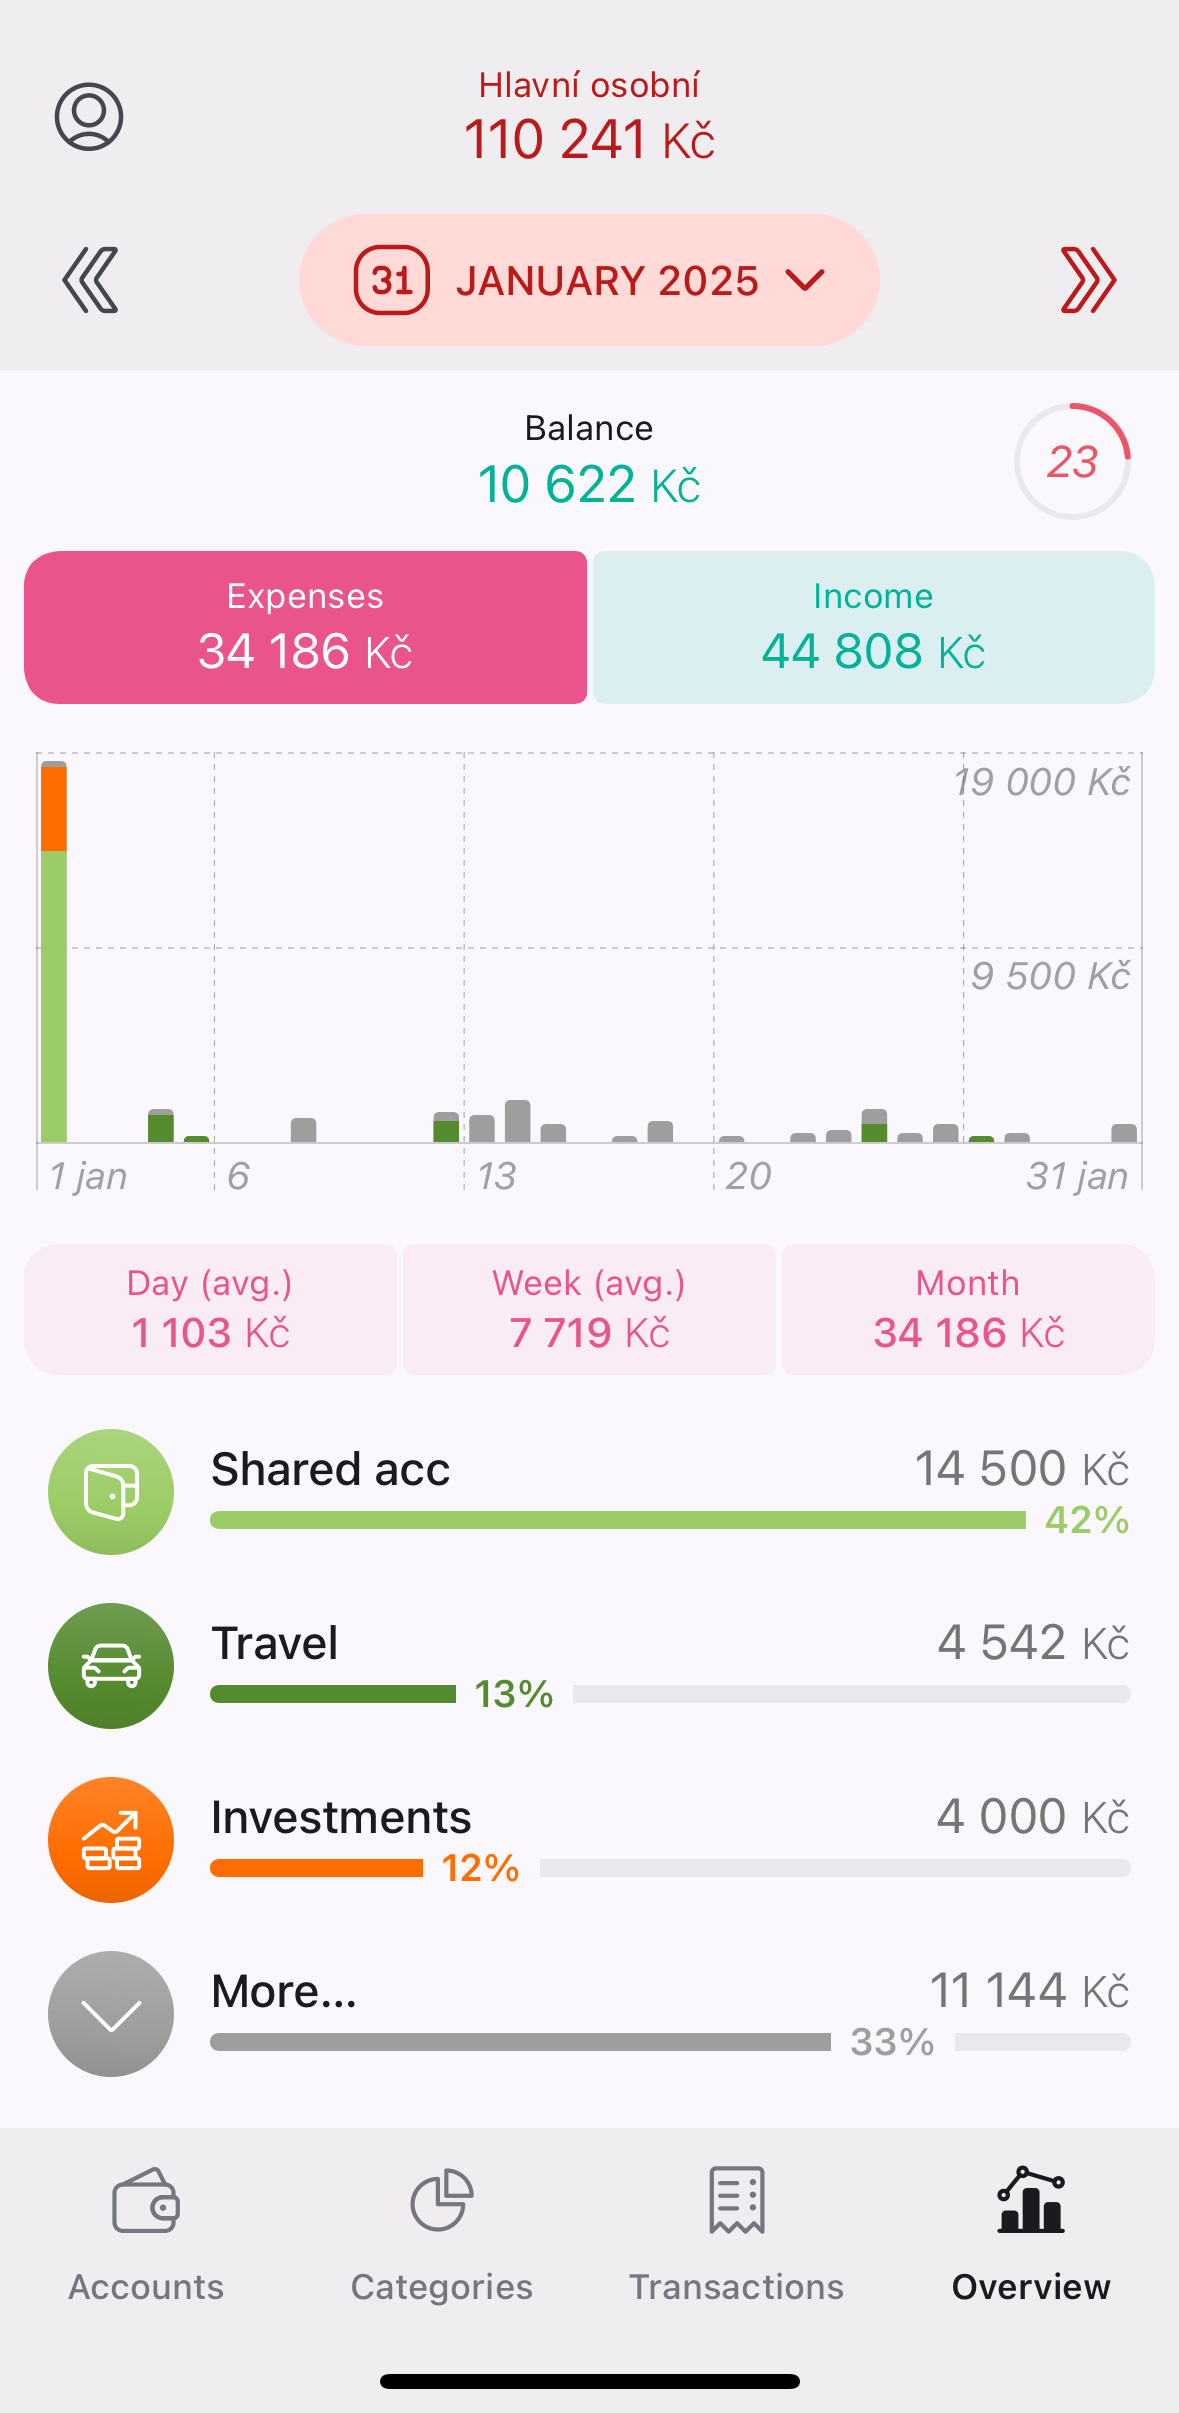
\includegraphics[width=0.35\textwidth]{images/onemoney1.PNG}
    \hspace{10px}
    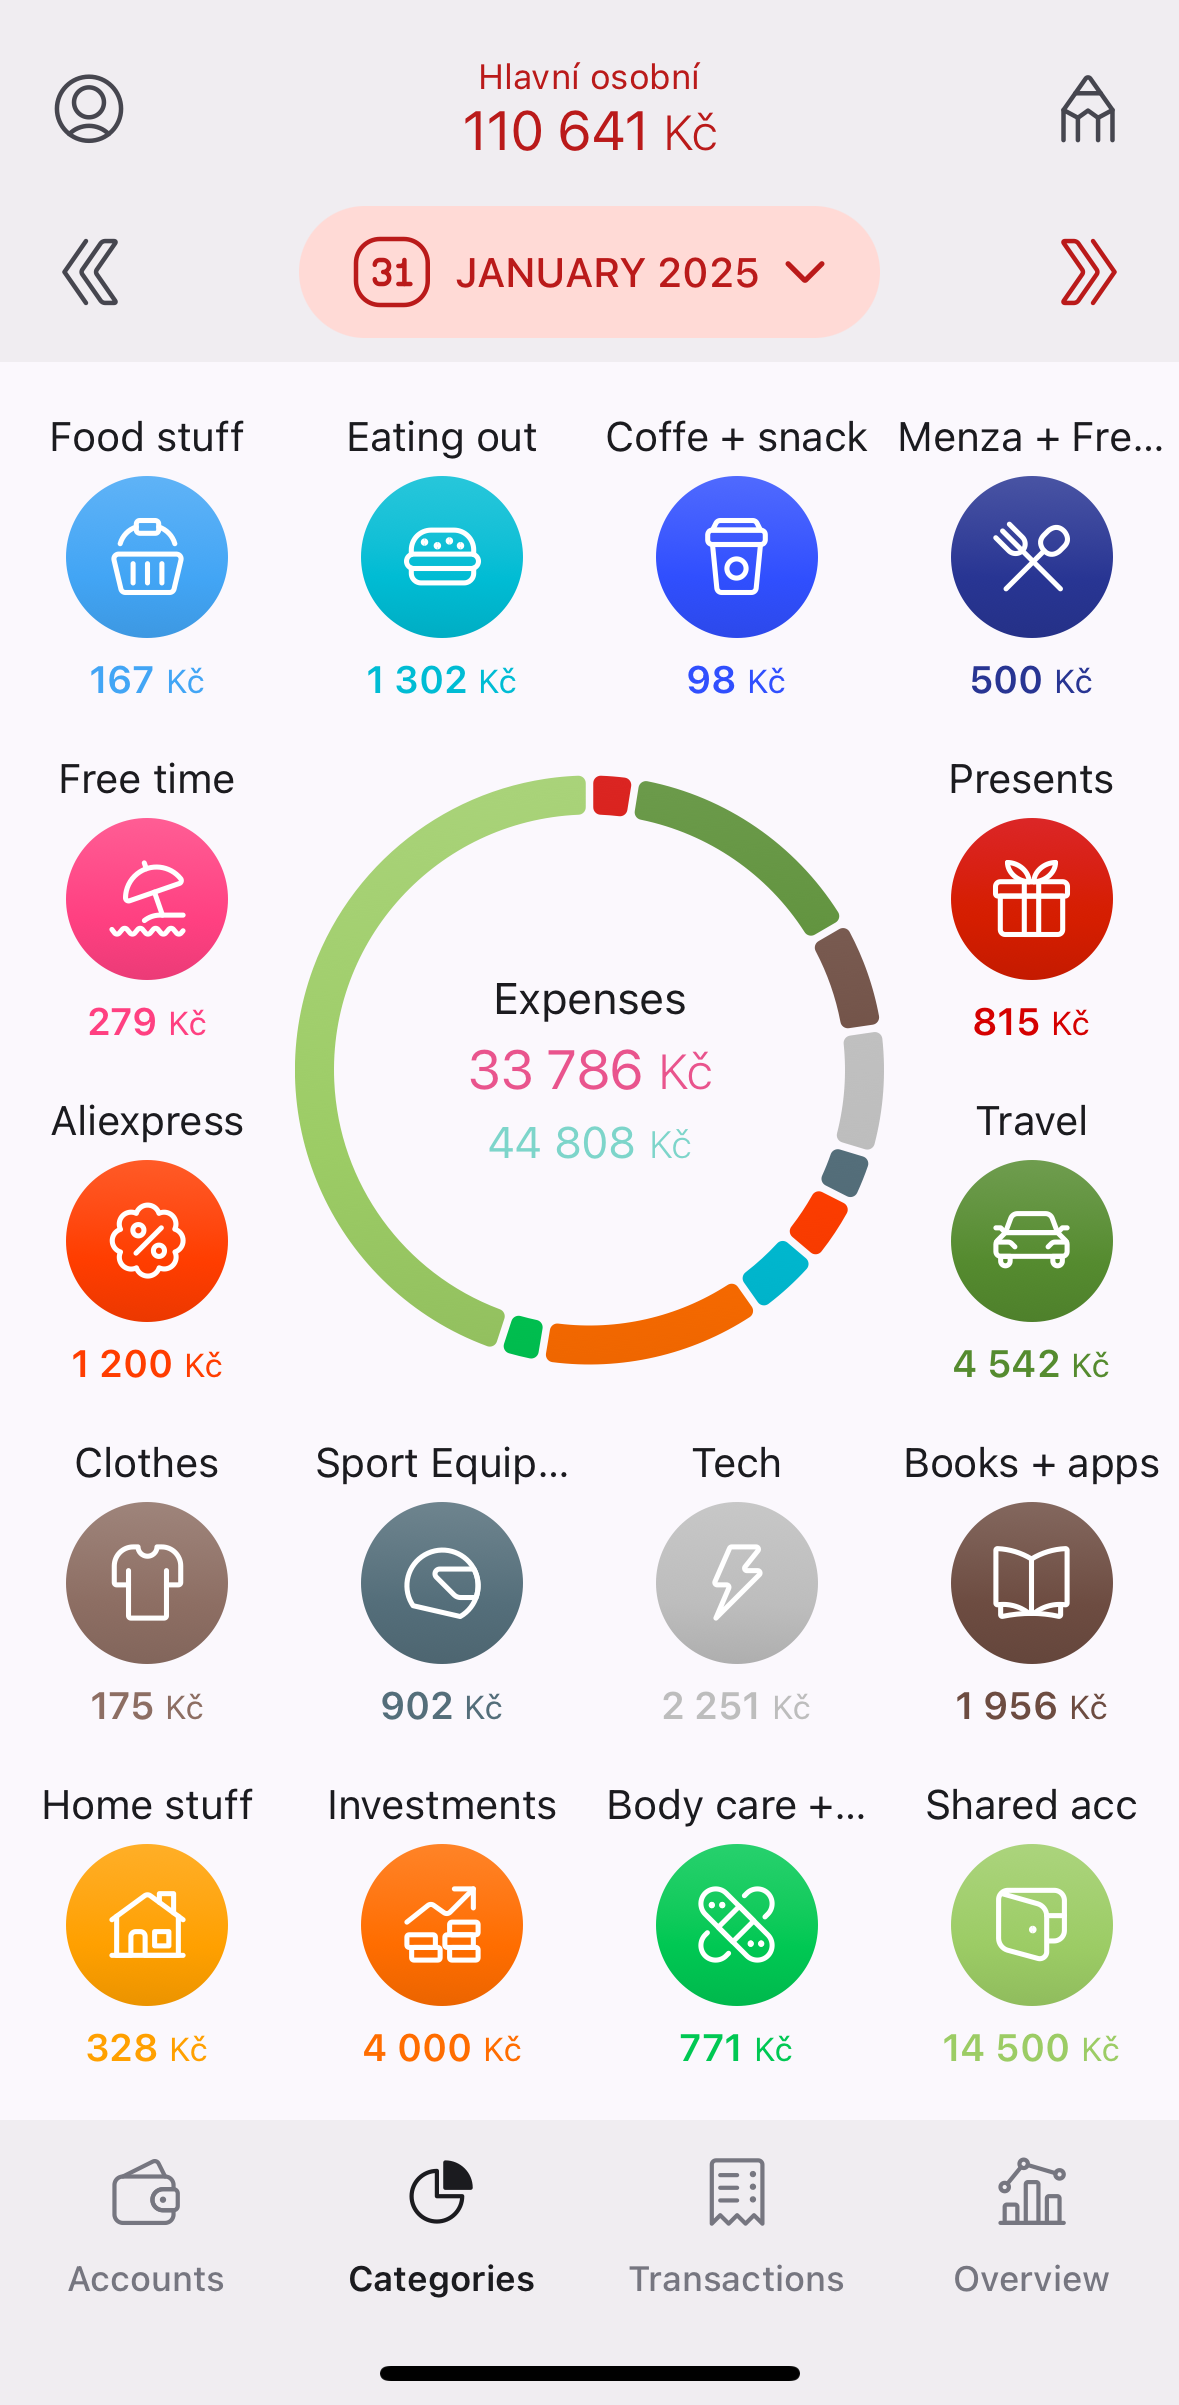
\includegraphics[width=0.35\textwidth]{images/onemoney2.PNG}
    \caption{Aplikace 1Money}
\end{figure}

\subsection{Cashew}
Multiplatformní aplikace založená na stejné technologii Flutter jako moje aplikace se jmenuje Cashew \cite{cashew}. Implementuje komponenty z Material Design, ale rozvržení obrazovky si autoři uspořádali podle sebe. Uživateli umožňuje široké možnosti nastavení z hlediska vzhledu (barvy, typ písma, typ ikon či formáty data i čísel). Umožňuje zálohování dat na Google disk i import z csv souborů. Podporuje funkci více účtů. Obsahuje i placenou verzi, které je primárně podporu pro vývojáře.

\begin{figure}
  \centering
    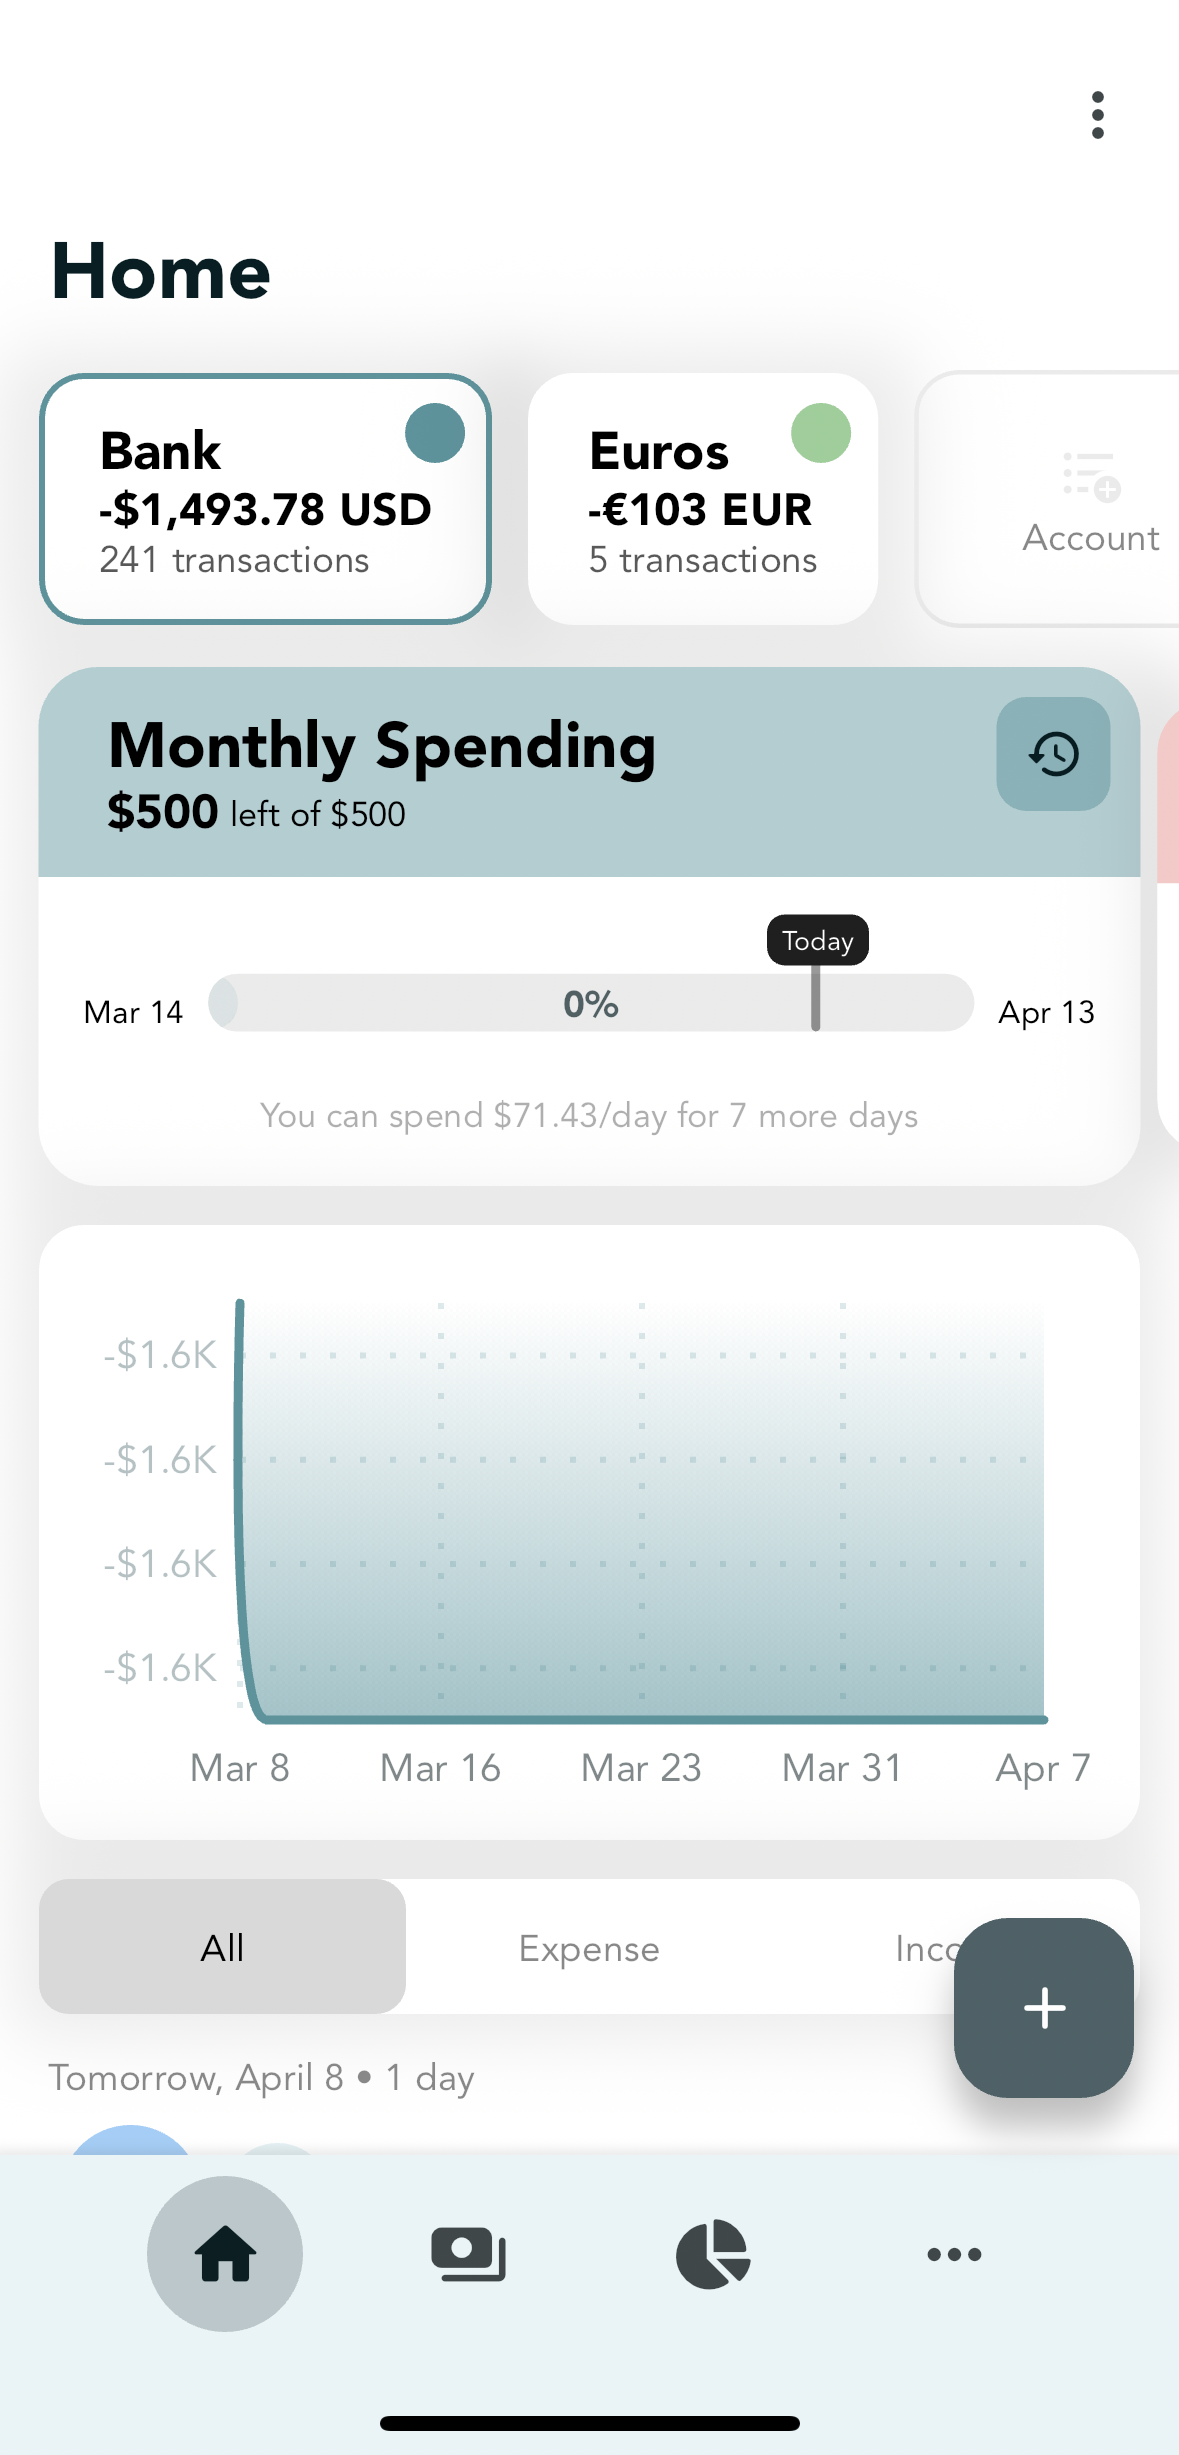
\includegraphics[width=0.35\textwidth]{images/cashew2.PNG}
    \hspace{10px}
    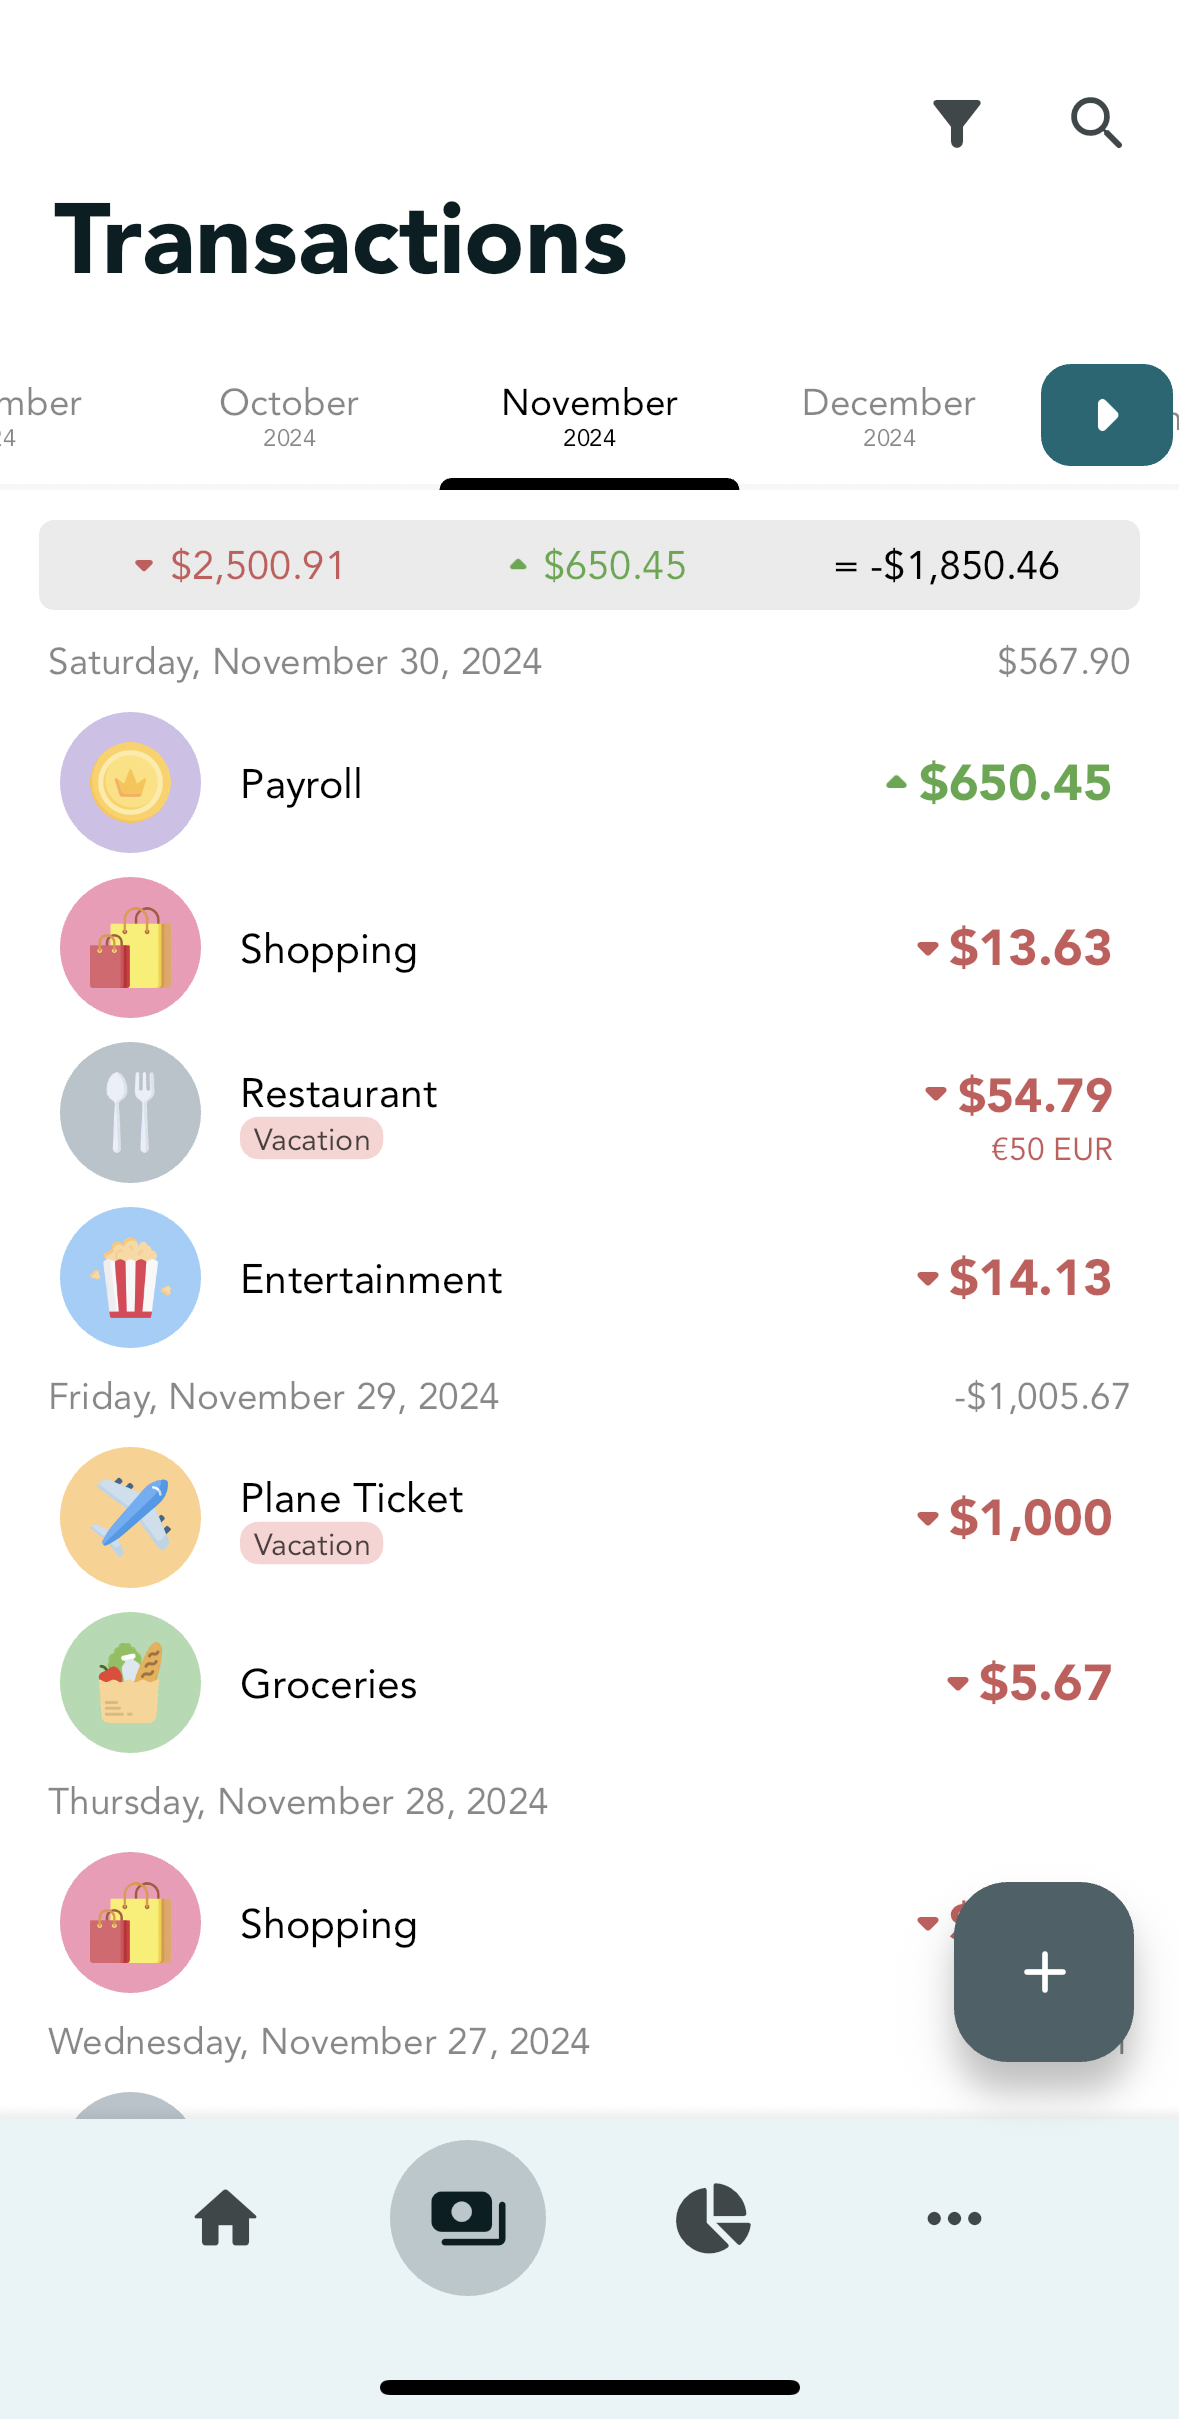
\includegraphics[width=0.35\textwidth]{images/cashew1.PNG}
  \caption{Aplikace Cashew}
\end{figure}

\subsection{Wallet}
Mobilní aplikace Wallet \cite{wallet} je dostupná na platformy Android i iOS. Za její stažení uživatel v první fázi nezaplatí. Nabízí všechny základní funkce, co by uživatel očekával -- kategorie transakcí, podpora více měn, přidání poznámky. Z hlediska analýzy a grafového zobrazení je na výběr jen velmi málo možností v z mého pohledu nepřehledném uspořádání. Ze zajímavých funkcionalit stojí za zmínku plánované transakce nebo automatická bankovní synchronizace (tato funkce je už placená).

\begin{figure}
  \centering
  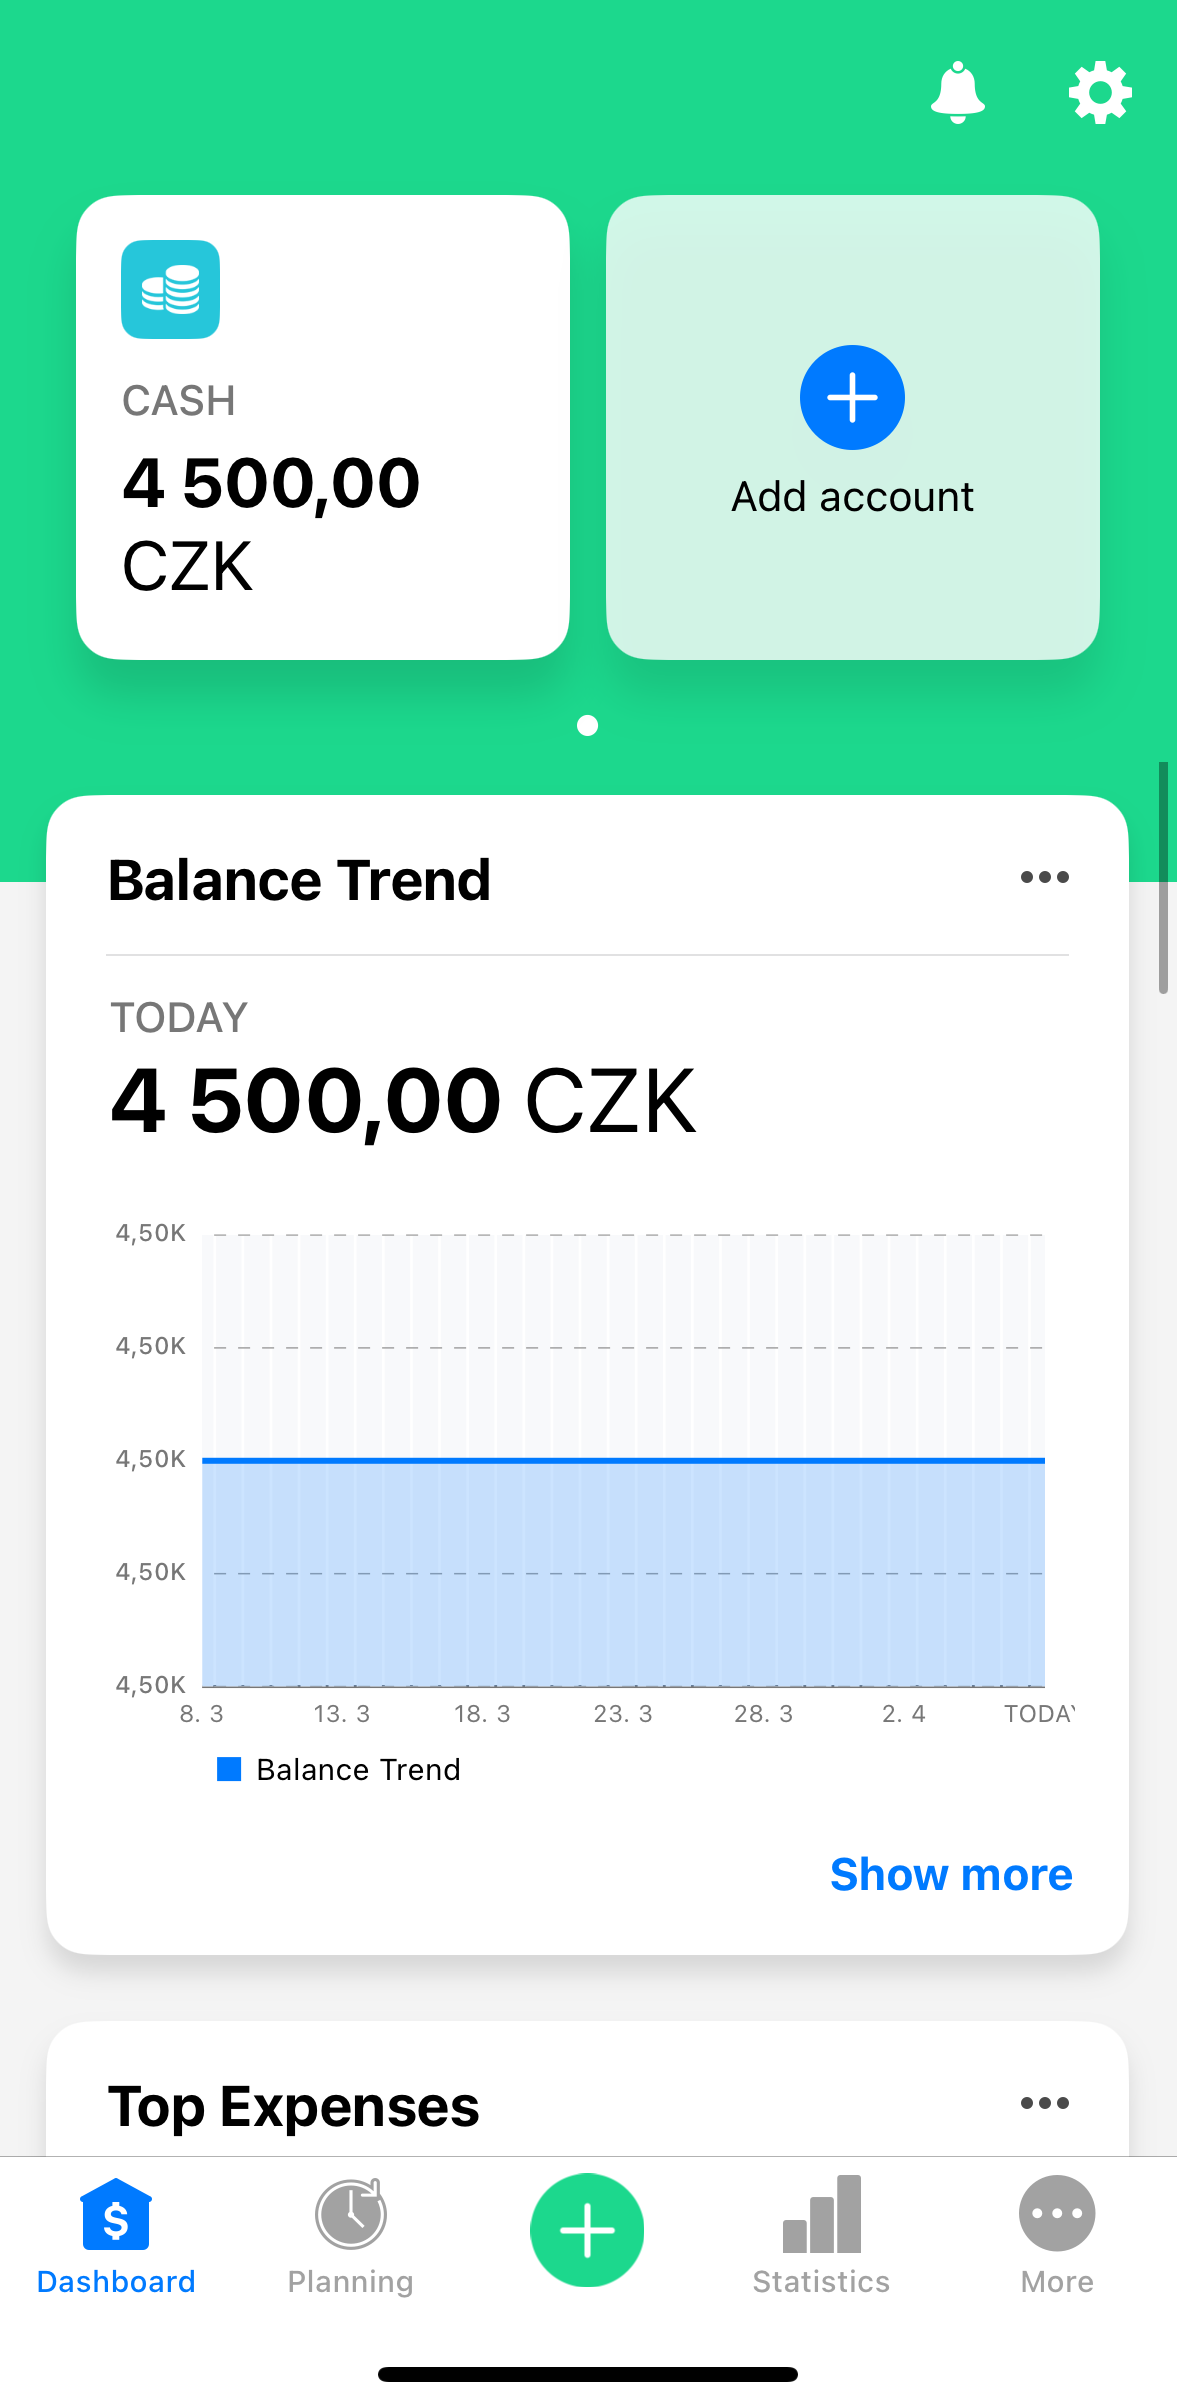
\includegraphics[width=0.35\textwidth]{images/wallet1.PNG}
    \hspace{10px}
    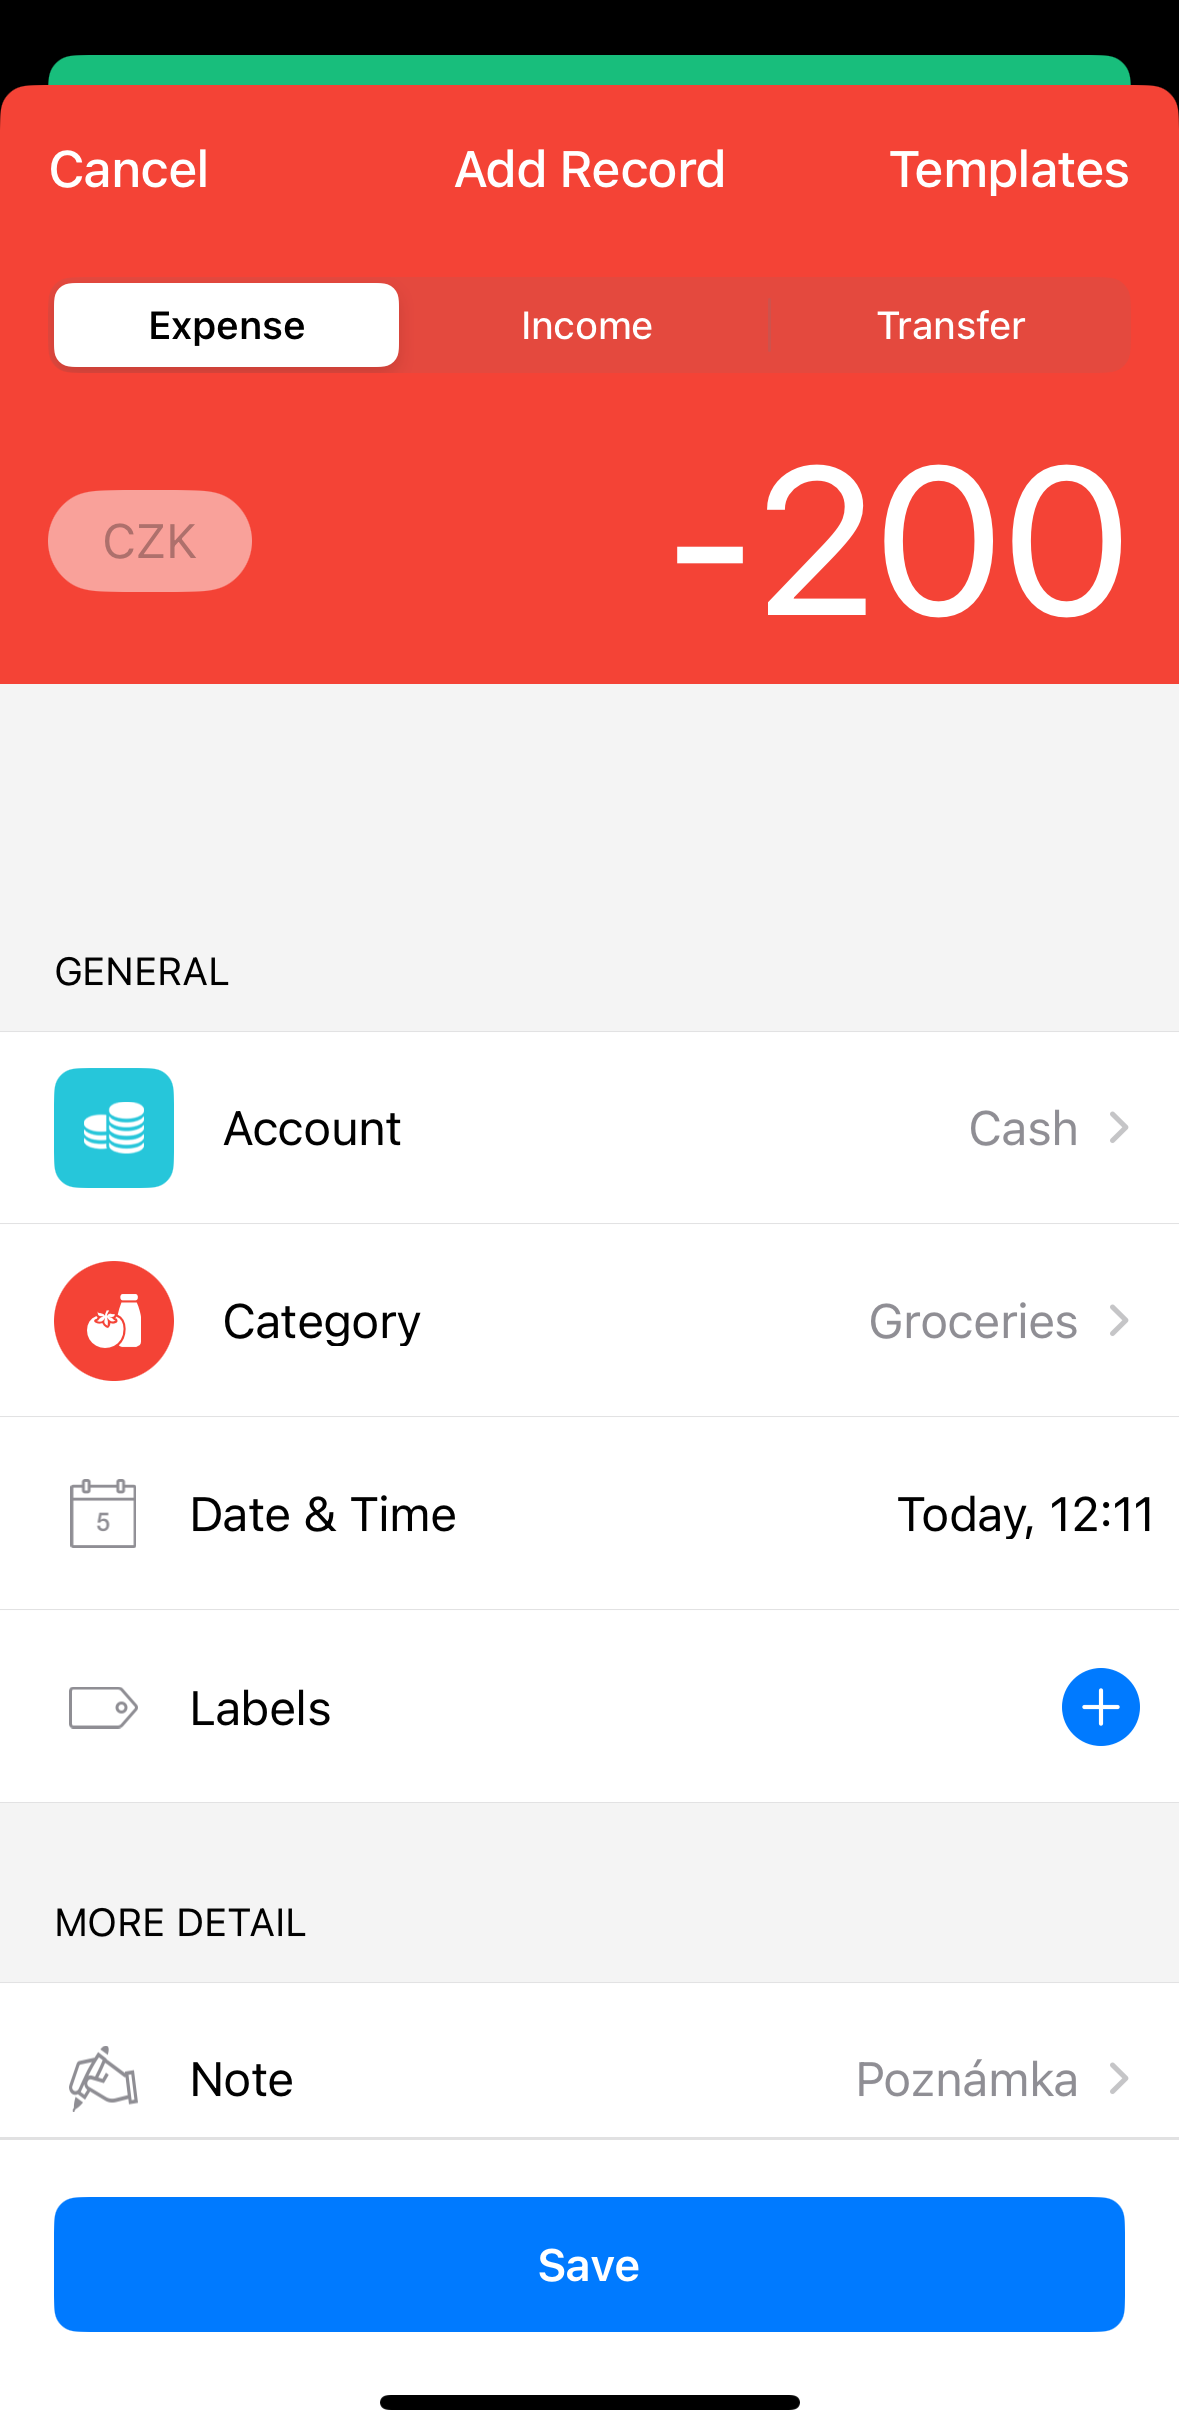
\includegraphics[width=0.35\textwidth]{images/wallet2.PNG}
  \caption{Aplikace Wallet}
\end{figure}

\subsection{Money Manager Ex}
Aplikace dostupná jak na mobilní zařízení (nízký počet stažení \cite{money-manager-android}) tak především i na desktopové zařízení \cite{money-manager}. Uživatelské rozhraní je na první pohled relativně přívětivé, i když místy obsahuje širokou škálu tlačítek a možností k nastavení. Při prvním spuštění nevyžaduje žádné složité nastavení. Zde se mi velmi líbí velká nabídka grafů k analýze údajů a možnost exportu do PDF pro většinu obrazovek.

\begin{figure}
  \centering
  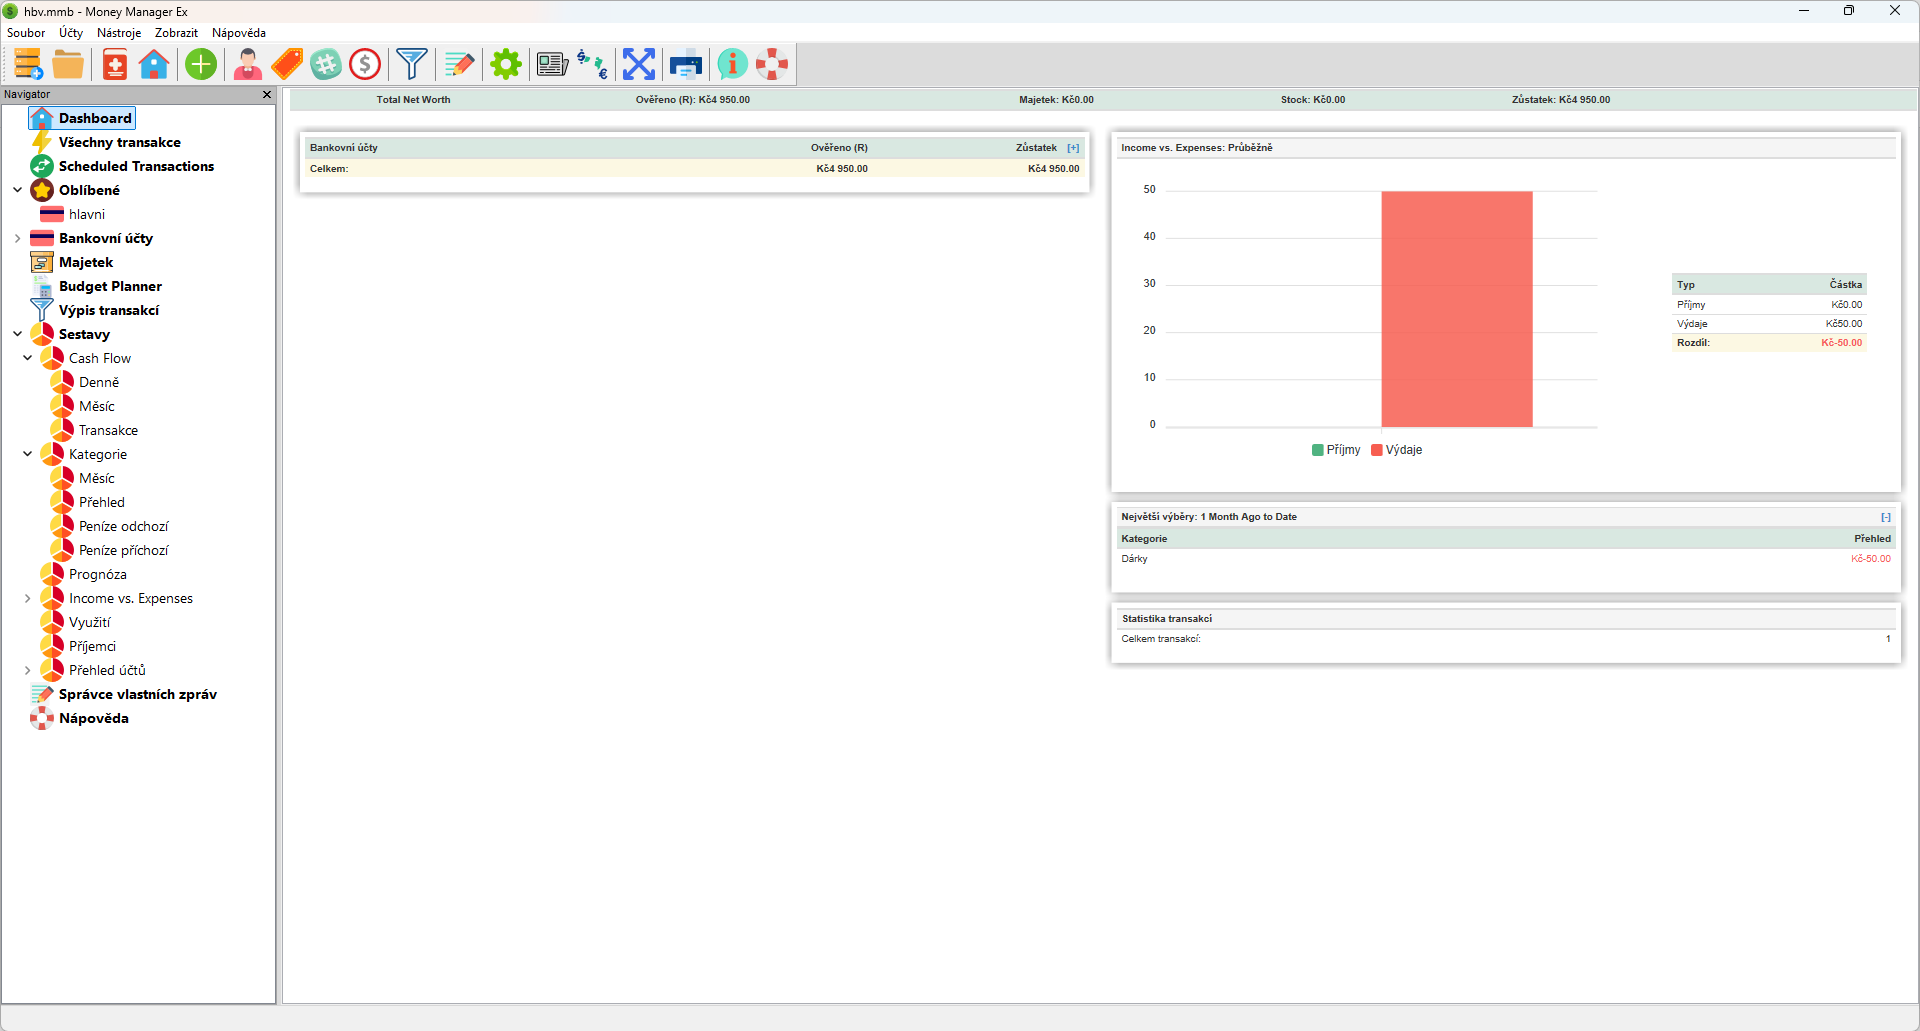
\includegraphics[width=1\textwidth]{images/manager-ex.png}
  \caption{Aplikace Money Manager Ex}
\end{figure}

\subsection{Homebank}
Desktopová aplikace dostupná na Windows, Linux i macOS \cite{homebank}. Z hlediska uživatelského komfortu je oproti Money Manager Ex jednodušší na používání. Při prvotním nastavení sice člověk musí vhodně nakonfigurovat svůj účet, v~dalších fázích je už používání intuitivní. Centrem aplikace je obrazovka se stavy účtu, přehledem transakcí a jednoduchými grafy. Všechny ostatní funkce se pak otevírají jako nové okno. Uživatelské rozhraní působí moderním a intuitivním dojmem.

\begin{figure}
  \centering
  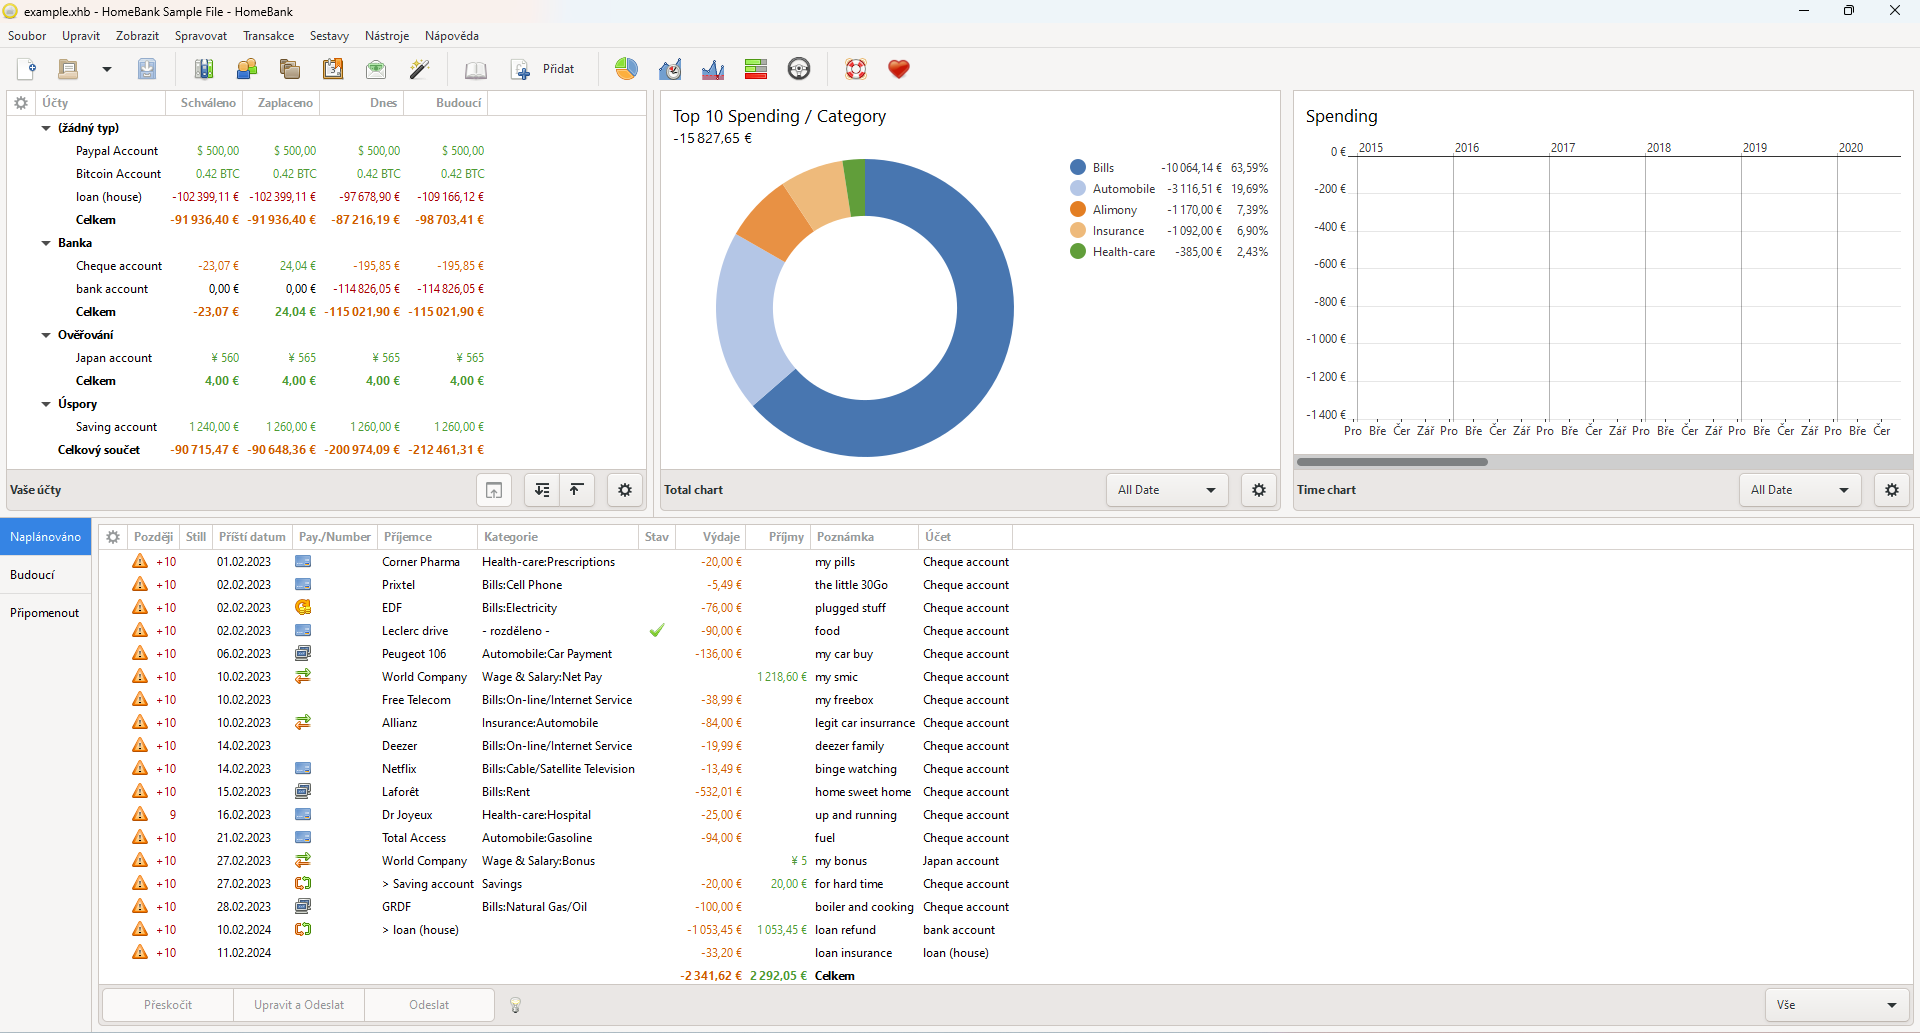
\includegraphics[width=1\textwidth]{images/homebank.png}
  \caption{Aplikace Homebank}
\end{figure}

Oproti existujícím aplikacím by tato měla nabídnout přívětivější uživatelské rozhraní a ulehčit první použití. Rád bych přinesl i lepší vizualizaci v podobě grafů a zajímavých číselných údajů. V neposlední řadě by měla být spustitelná na libovolné platformně, tak aby uživatel nebyl limitován například při změně mobilního telefonu.

\section{Použité technologie}

Požadavkem byla multiplatformní vývoj existuje řada technologií \cite{jetbrains-crossplatform}, které však k tvorbě aplikace přistupují odlišným způsobem. Mezi nejpopulárnější technologie vhodné na tuto práci se řadí \textit{React Native} a \textit{Flutter}. Jelikož jsem za dobu, co se věnuji programování nepřilnul k webovým technologiím, na kterých primárně stojí React Native, zvolil jsem Flutter. Přispěl k tomu fakt, že se více blíží klasickým objektově orientovaným jazykům a jednoduše implementuje \textit{Material Design}, který rád v uživatelském rozhraní vídám.

Aplikace je otestována a řádně funguje na obou mobilních platformách (Android iOS) a jako desktopová Windows aplikace. Ze stejného kódu jde sestavit i aplikace na macOS a Linux. Tyto platformy jsem však netestoval a nemohu zaručit jejich bezproblémový chod.

\subsection{Dart}
Objektově orientovaný jazyk Dart \cite{dart} pochází od společnosti Google, jehož první verze byla zveřejněna 14. listopadu 2013. Momentálně je jeho aktuální verze 3. Jde o typově bezpečný jazyk, podporující třídy se syntaxí založenou na jazyku C. Může být kompilován do strojového kódu, jazyky JavaScript nebo WebAssembly. Taktéž je základem pro framework Flutter.

\kiinlinecode{}{;}
Je dodáván se širokou škálou základních knihoven, které umožňují obstarat běžný vývoj. Jako příklad mohu uvést knihovnu \kiinlinecode{}{;}{dart:async}, která umožňuje asynchronní programování za využití tříd jako je \kiinlinecode{}{;}{Future} nebo knihovna \kiinlinecode{}{;}{dart:io} pro práci se souborovým systémem či HTTP protokolem.

Technologie jazyka Dart umožňují spustit kód dvěma způsoby. První z nich je určen pro mobilní a desktopové aplikace. Dart obsahuje virtuální stroj s JIT\footnote{Just in time} kompilací, který se používá především ve fázi vývoje. Tento způsob umožňuje tzv. inkrementální rekompilaci jejíž výhodou je funkcionalita \textit{hot reload} či nástroje \textit{DevTools} pro aktuální metriky ladění. Dále i AOT\footnote{Ahead of time} kompilátor pro tvorbu strojového kódu, který se využívá při sestavování apliakce pro použití v produkci. Druhý způsob se týká webové platformy, kde Dart umožňuje kód přeložit do JavaScript nebo WebAssembly. Opět i zde Dart využívá různé techniky pro ladění kódu a následné produkci. Oba tyto způsoby jsou stejné v tom že potřebují \textit{běhové prostředí Dart}. Toto prostředí se stará o správu paměti pomocí garbage collector, vynucení kontroly typů a správu vláken.

\begin{kicode}{}{}{Ukázka kódu v jazyce Dart}
class Point {
  final double x;
  final double y;

  const Point(this.x, this.y);

  bool get isInsideUnitCircle => x * x + y * y <= 1;
}
\end{kicode}

\subsection{Flutter}
Open source framework Flutter \cite{flutter} slouží pro tvorbu uživatelských Využívá Dart a je taktéž vyvíjený společností Google. Poprvé zveřejněn byl v květnu 2017. Google sám ho využívá v aplikacích jako je Google Play nebo Goole Earth \cite{flutter-showcase}. Mezi nejznámější aplikace třetích stran používajících Flutter patří Alibaba nebo hra PUBG Mobile \cite{flutter-showcase}.

Používá své vlastní vykreslovací jádro, které pixely přímo vykresluje na obrazovku. Toto je podstatný rozdíl oproti řadě jiných frameworků, které se spoléhají na vykreslovací jádro dané platformy. Tento přístup umožňuje mít identicky vypadající uživatelské rozhraní napříč všemi podporovanými platformami.

Základní komponentou je \textit{widget}. Ten se dále může skládat z dalších widgetů. Celé uživatelské rozhraní je poté poskládáno z těchto celků. Flutter sám o sobě poskytuje dva typy předdefinovaných widgetů -- Material Design (viz kapitola \ref{material-design}) widgety a Cupertino widgety. Přestože oba mají svoji primární platformu, Flutter je umožňuje používat libovolně kdekoliv. Programátor si samozřejmě sám může definovat widgety vlastní.

Pro rozložení prvků na stránce (vytvoření \textit{layout}) se taktéž používají widgety, přestože nejsou při zobrazení viditelné. Základními widgety pro tvorbu layoutu jsou \kiinlinecode{}{;}{Row}, \kiinlinecode{}{;}{Column} a \kiinlinecode{}{;}{Container}. Pomocí \kiinlinecode{}{;}{Container} můžeme ostatním widgetům přidávat odsazení atd. Tyto widgety slouží pro specifickou či nízkoúrovňovou tvorbu layoutu. Můžeme využít i specializované widgety jako \kiinlinecode{}{;}{GridView} pro tvorbu mřížky nebo \kiinlinecode{}{;}{ListView} pro rolovatelný seznam. Nejvíce specifické widgety jako \kiinlinecode{}{;}{BottomNavigationBar} či \kiinlinecode{}{;}{AppBar} zajistí dodržení pravidel stanovených Material Designem a umožní programátorovi velmi jednoduchou implementaci.

\subsection{Material Design} \label{material-design}
V březnu 2025 je Material Design verze 3 \cite{m3} nejnovějším open source designový systém od společnosti Google. Systémem v tomto případě mám na mysli soubor pravidel pro uživatelské rozhraní, konkrétní komponenty i barevné provedení. Všechny tyto prvky jsou vytvořeny zkušenými designéry s respektem pro psychologický vliv uživatelského rozhraní na člověka.

Předchozí označení verze 3 napovídá, že v minulosti již proběhly aktualizace tohoto systému. Tento krok dává smysl vzhledem k vyvíjejícím se trendům v~oblasti designu. Tyto aktualizace mohl běžných uživatel pozorovat v operačním systému Android nebo v aplikacích od Googlu, jelikož Google tento systém používá téměř všude.

Použití tohoto systému má ve Flutteru řadu výhod. Především většina Material widgetů je již implementována \cite{m3-components} a použití programátorem je velmi jednoduché. Programátor nemusí často řešit rozmístění jednotlivých prvků v konkrétní komponentě ani správnou adaptaci na velikost zařízení. Běžnou součástí aplikací jsou ikony. Ikony z Material Designu jsou ve Flutteru k přímému použití bez specifického nastavení. Programátor nemusí řešit žádné externí SVG soubory. Stejně to platí i pro použití fontů písem.

\subsection{SQLite}
SQLite \cite{sqlite} je velmi jednoduchá a rychlá relační databáze, která je uložena v jediném souboru. Vývoj SQLite byl zahájen v roce 2000. Obvykle jsou všechny potřebné závislosti již zabudovány v zařízeních, ať už jde o mobilní telefony nebo desktopové operační systémy. Je zdarma k užití pro libovolné účely. Přesto poskytuje plnohodnotnou SQL implementaci. Zajímavostí je, že onen soubor je multiplatformní. Nevadí mu přenos mezi 32bitovými a 64bitovými systémy nebo architekturami big-endian a little-endian.

\subsection{Balíčky}

Přestože balíčky tvoří závislosti projektu na ostatních okolnostech a programátor se musí spoléhat na jiné programátory, že je budou udržovat aktuální, je nemožné se jim v dnešním době vyhnout. Dart a Flutter má výběr z široké veřejné knihovny balíčků, které jsou vyvíjeny ostatními programátory. Balíčky je nutné do projektu zahrnout. Celý jejich seznam je dostupný v~souboru \kiinlinecode{}{;}{pubspec.yaml}. 

\begin{itemize}
  \item \textbf{Drift} \cite{drift} je balíček poskytující rozhraní pro práci s SQLite databází. Její velkou výhodou oproti ostatním implementacím SQLite pro Dart je možnost multiplatformnosti. Funguje na všech platformách od Androidu přes Windows až po webové rozhraní. V oficiálním návodu je doporučena knihovna sqflite, ta však tuto výhodu neposkytuje. Dále poskytuje velmi jednoduché API pro vytváření dotazů nad databází bez použití jazyka SQL. Programátor vytváří strukturu databáze v jednom souboru, na jehož základě si Drift generuje interní soubory.
  \item \textbf{GoRouter} \cite{gorouter}je deklarativní balíček pro organizaci navigace v rámci aplikace (tzv. \textit{routování}). Funguje na principu URL adres. Umožňuje v adrese předávat parametry, zajistit přesměrování na základě práv uživatele či použití \textit{vnitřních navigátorů} nejčastěji pro komponentu \kiinlinecode{}{;}{BottomNavigationBar}, který zůstává neustále viditelný skrz více obrazovek. Pro přechody umožňuje nastavit vlastní libovolné animace. Výhodou je, že autorem jsou přímo oficiální vývojáři Flutter, tudíž by balíček měl zůstat udržovaný.
  \item \textbf{Skeletonizer} \cite{skeletonizer} zjednodušeným způsobem poskytuje funkcionalitu označovanou jako \textit{skeleton loading}. Používá se při načítání obsahu na stránce a zobrazuje hrubý náhled rozložení prvků na stránce. Vše je doplněno vhodnou animací, aby uživatel ihned poznal, že se obrazovka právě načítá. Zjednodušení použitím tohoto balíčku spočívá v tom, že programátorovi stačí již definovaný widget \uv{obalit} widgetem \kiinlinecode{}{;}{Skeletonizer} z tohoto balíčku a o zbytek práce se balíček postará sám.
  
  \begin{figure}
  	\centering
  	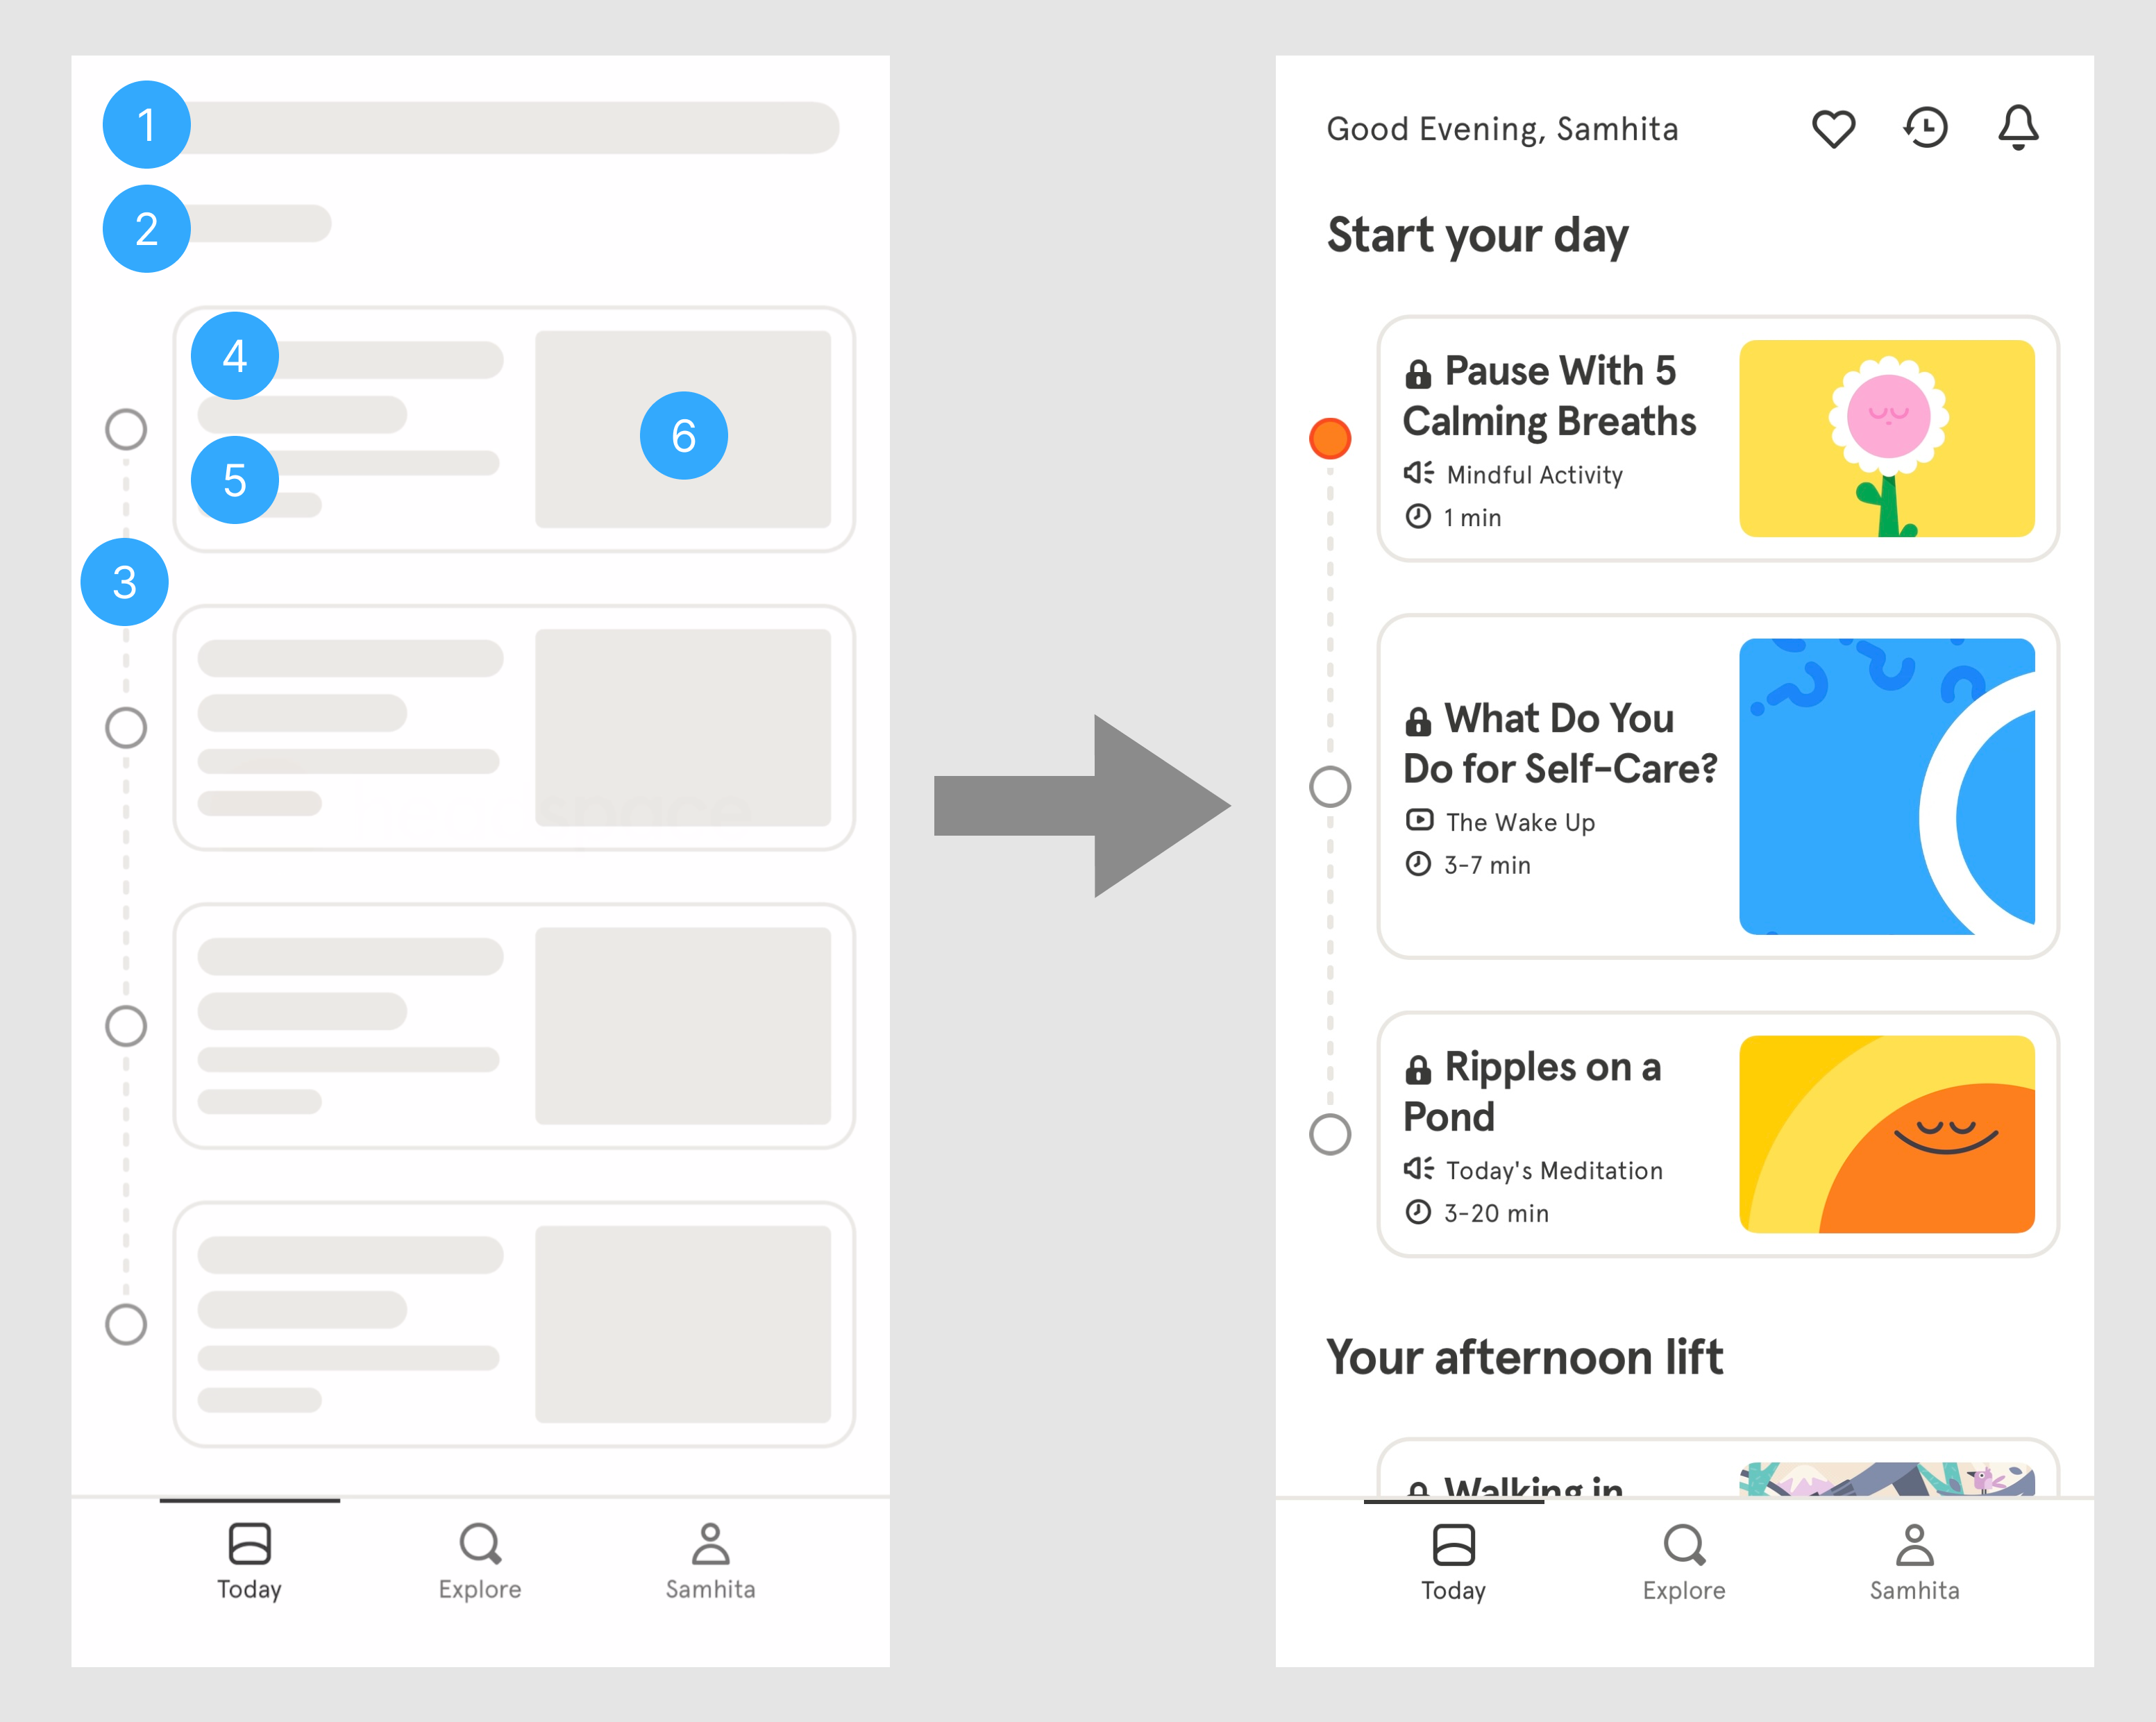
\includegraphics[scale=0.1]{images/skeletonizer.png}
  	\caption{Skeleton loading a načtená obrazovka - převzato z \cite{skeleton}}
  \end{figure}
  
  \item \textbf{Another Flushbar} \cite{flushbar} poskytuje vylepšenou komponentu \kiinlinecode{}{;}{Snackbar} z Material Design. Účelem komponenty je krátce informovat uživatele o akci, která byla právě provedena. Obvykle se objevuje ve spodní části obrazovky. Vylepšení spočítá v možnosti většího přizpůsobením - přidání ikony, změna barvy či animace a libovolné umístění. Já tento balíček preferoval i z důvodu správného zobrazování při otevřeném dialogovém okně.

\begin{figure}
	\centering
	
\includegraphics[width=0.5\textwidth]{images/flushbar.pdf}
	\caption{Komponenta Flushbar}
\end{figure}
    
    
  \item \textbf{Syncfusion Flutter Charts} \cite{syncfusion-charts} je rozsáhlá knihovna pro tvorbu grafů. Umožňuje vytvářet všechny druhy grafů - sloupcové, spojnicové, prstencové a další (autoři uvádí více než 30 druhů). Grafy lze dále přizpůsobovat - výběr animace, úprav jednotek na osách, výběr barev, možnost zobrazit legendu či podrobné informace daného bodu v grafu po přejetí myší. Přes širokou škálu úprav je základní použití velmi jednoduché. Velkým bonusem je rozsáhlá dokumentace s ukázkami všech typů grafů a jejich zdrojových kódů.
  \item \textbf{File Picker} \cite{file-picker} dává programátorovi možnost využít nativní průzkumník souborů k výběru složky nebo konkrétních souborů pro jejich další zpracování v aplikaci. Je možnost soubory filtrovat či umožnit výběr více z nich najednou. Základní funkcionalitu poskytuje na libovolné platformně s velmi jednoduchou implementací. V mém případě jsem ho použil pro výběr složky, kam si uživatel chce uložit exportované soubory. 

\end{itemize}


\section{Programátorská příručka}

Multiplatformní vývoj přináší jistá specifika (nutnost zvolit vhodné technologie, nutnost případné optimalizace zobrazení či zúžený výběr knihoven), ale z hlediska architektury či samotného procesu programování je většina věcí stejných. Zvolená technologie často sama navádí k použití vhodných prvků.

Mnou navržené a vytvořené aplikace jsem dal název Budget Buddy. Je určena pro mobilní telefony, tablety i desktopová zařízení. Testování probíhalo na operačních systémech Android verze xx a vyšší, iOS xx a vyšší a Windows xx a vyšší. Pro ostatní operační systémy není zaručena plná funkcionalita, i když z podstaty frameworku by se tak stát nemělo.

Pro vývoj aplikace jsem použil textový editor Visual Studio Code s řadou rozšíření. Část práce specifické pro platformu Android jsem realizoval v prostředí Android Studio. Především se jednalo o úlohy typu aktualizace Software Developement Kit či migrace na novější verzi Kotlin gradle, kde Androi Studio poskytuje jednodušší rozhraní a programátora výborně provede celým procesem.

\subsection{Architektura aplikace}
Pro multiplatformní vývoj neexistuje doporučená architektura už z podstaty věci širokého záběru různých zařízení. Je možné se držet dlouho známých architektur, které se používají v různých systémech (\textit{Model-View-Controller} či \textit{Mode-View-Viewmodel}) nebo se řídit podle zvyklostí daného frameworku (ve Flutteru se jedná například o \textit{The Clen Architecture} nebo \textit{Bloc}). Já se ve své aplikaci držel architektury Model-View-Viewmodel, jelikož s ní mám z minulosti zkušenosti a pro moji malou aplikaci je plně dostačující. 

Model-View-Viewmodel (zkráceně MVVM) je architektura, která odděluje v aplikaci uživatelské rozhraní, logiku a datovou část \cite{mvvm}. Ve Flutteru je velmi dobře podporována, jednak z hlediska komponent frameworku, tak i ofociální dokumentace na architekturu odkazuje jako vhodný příklad návrhu aplikace. Rozdělení aplikace je do následujících tří detailněji popsaných celků.
\begin{itemize}
  \item \textbf{Model} je částí zapouzdřující data, se kterými aplikace pracuje. Udává strukturu poskytovaných dat i metody pro jejich získání objekty ve Viewmodel.
  \item \textbf{View} je zodpovědné za strukturu a zobrazení uživatelského rozhraní. Neměl by obsahovat žádnou logiku aplikace. Vstupy které přijme od uživatele předává ke zpracování na Viewmodel. 
  \item \textbf{Viewmodel} je prostředníkem mezi View a Model. Do View poskytuje data a případně je upraví do vhodného formátu pro zobrazení. Reaguje na zprávy od View, které představují vstupy uživatele. Vlákno pro uživatelské rozhraní by neměl blokovat, zlepší se tím uživatelský zážitek.
\end{itemize}

V mé konkrétní implementaci je kód strukturován do složek podle MVVM architektury - \kiinlinecode{}{;}{model}, \kiinlinecode{}{;}{view} a \kiinlinecode{}{;}{view_model}. Ve \kiinlinecode{}{;}{view} je jemnější rozdělení na obrazovky \kiinlinecode{}{;}{screens} a jednotlivé widgety \kiinlinecode{}{;}{widgets}. Dále je v projektu i složka \kiinlinecode{}{;}{data} pro databázi, složka \kiinlinecode{}{;}{utils} pro jednoduché funkce používané skrz projektem (převod kódu ikony na Ikonu, zkrášlení číselného formátu a další) a složka \kiinlinecode{}{;}{theme} spravuje vizuální téma aplikace.

\subsection{Multiplatformní část projektu}
Tady nevím jestli něco přesně bude, nebo cca co.

\subsection{Uchovávání stavu}
Uchování stavu jednotlivých obrazovek a jiných prvků je velmi důležité pro uživatelský komfort. Běžně se uživatel překlikne nebo přeskakuje mezi obrazovkami a nemá po každé změně vše nastavovat znovu nebo scrollovat na stejné místo v seznamu. Použití GoRouter za programátora řeší i tento problém. Není nutné nic nastavovat a stačí řídit se dokumentací GoRouter. Po zavedení do aplikace již uchování stavů funguje přesně tak, jak je pro uživatelský komfort vhodné. V~první řade bylo nutné vytvořit aplikaci konstruktorem s \kiinlinecode{}{;}{.router}. Do parametru \kiinlinecode{}{;}{router} jsem vložil konfiguraci GoRouter (viz kód \ref{gorouter-code}). V konfiguraci je uvedena cesta a obrazovka, která se při jejím zadání zobrazí.

\begin{kicode}{csharp}{gorouter-code}{Ukázka použití GoRouter}
  // GoRouter konfigurace
  final _router = GoRouter(
    routes: [
      GoRoute(
        path: '/',
        builder: (context, state) => HomeScreen(),
      ),
    ],
  );

  // konstruktor aplikace
  class MyApp extends StatelessWidget {
    @override
    Widget build(BuildContext context) {
      return MaterialApp.router(
        routerConfig: _router,
      );
    }
  }
\end{kicode}

\subsection{Implementace responzivního designu}
Responzivní design má zajistit, že aplikace se bude vhodně zobrazovat na libovolně velkém zařízení. Vyskytuje se především u webových technologií z důvodu běžného používání na různých typech zařízení. Stejná problemtika je u multiplatformních aplikací.

Podle velikosti obrazovky je nutné vhodně zvolit z určitých komponent, které slouží pro stejný účel, ale jsou jinak zobrazené. V této aplikace se jedná například o navigaci. Pro menší obrazovky jsem použil navigation bar, pro větší navigation rail, případně navigation drawer (viz obrázek \ref{pic-navigation}). Dále je nutné vhodně zobrazit komponenty v hlavním těle obrazovky. Řazení komponent na menším zařízení jsem zvolil pod sebe do sloupce, na větším naopak vedle sebe v řádku (viz obrázek grafy v mé appce). Je dostupná i komponenta \kiinlinecode{}{;}{GridView} vytvářející tabulku. Avšak není vhodná pro tvorbu layoutu. Material Design poskytuje i speciální kanonické rozložení (viz obrázek material), které je vhodné ve spojení se zobrazením seznamu. V této aplikaci by bylo vhodné pro obrazovku transakcí. Implementace pro Flutter zatím není dostupná, tudíž není možné ho použít. Dialogová okna jsem podle doporučení pro menší zařízení zvolil celoobrazovková, zatímco na větších jsou plovoucí (viz obrázek dialog okno moje).

Flutter poskytuje komponenty vhodné pro responzivní design, ale na programátorovi je ponecháno kdy jaké zvolí, včetně celé implementace. Zatím není dostupná žádná komponenta pro tvorbu responzivního rozložení, které by umožnila v jediném kódu pro uživatelské rozhraní rozhodnout do jakého widgetu kód \uv{obalit}.

\begin{figure}
  \centering 
  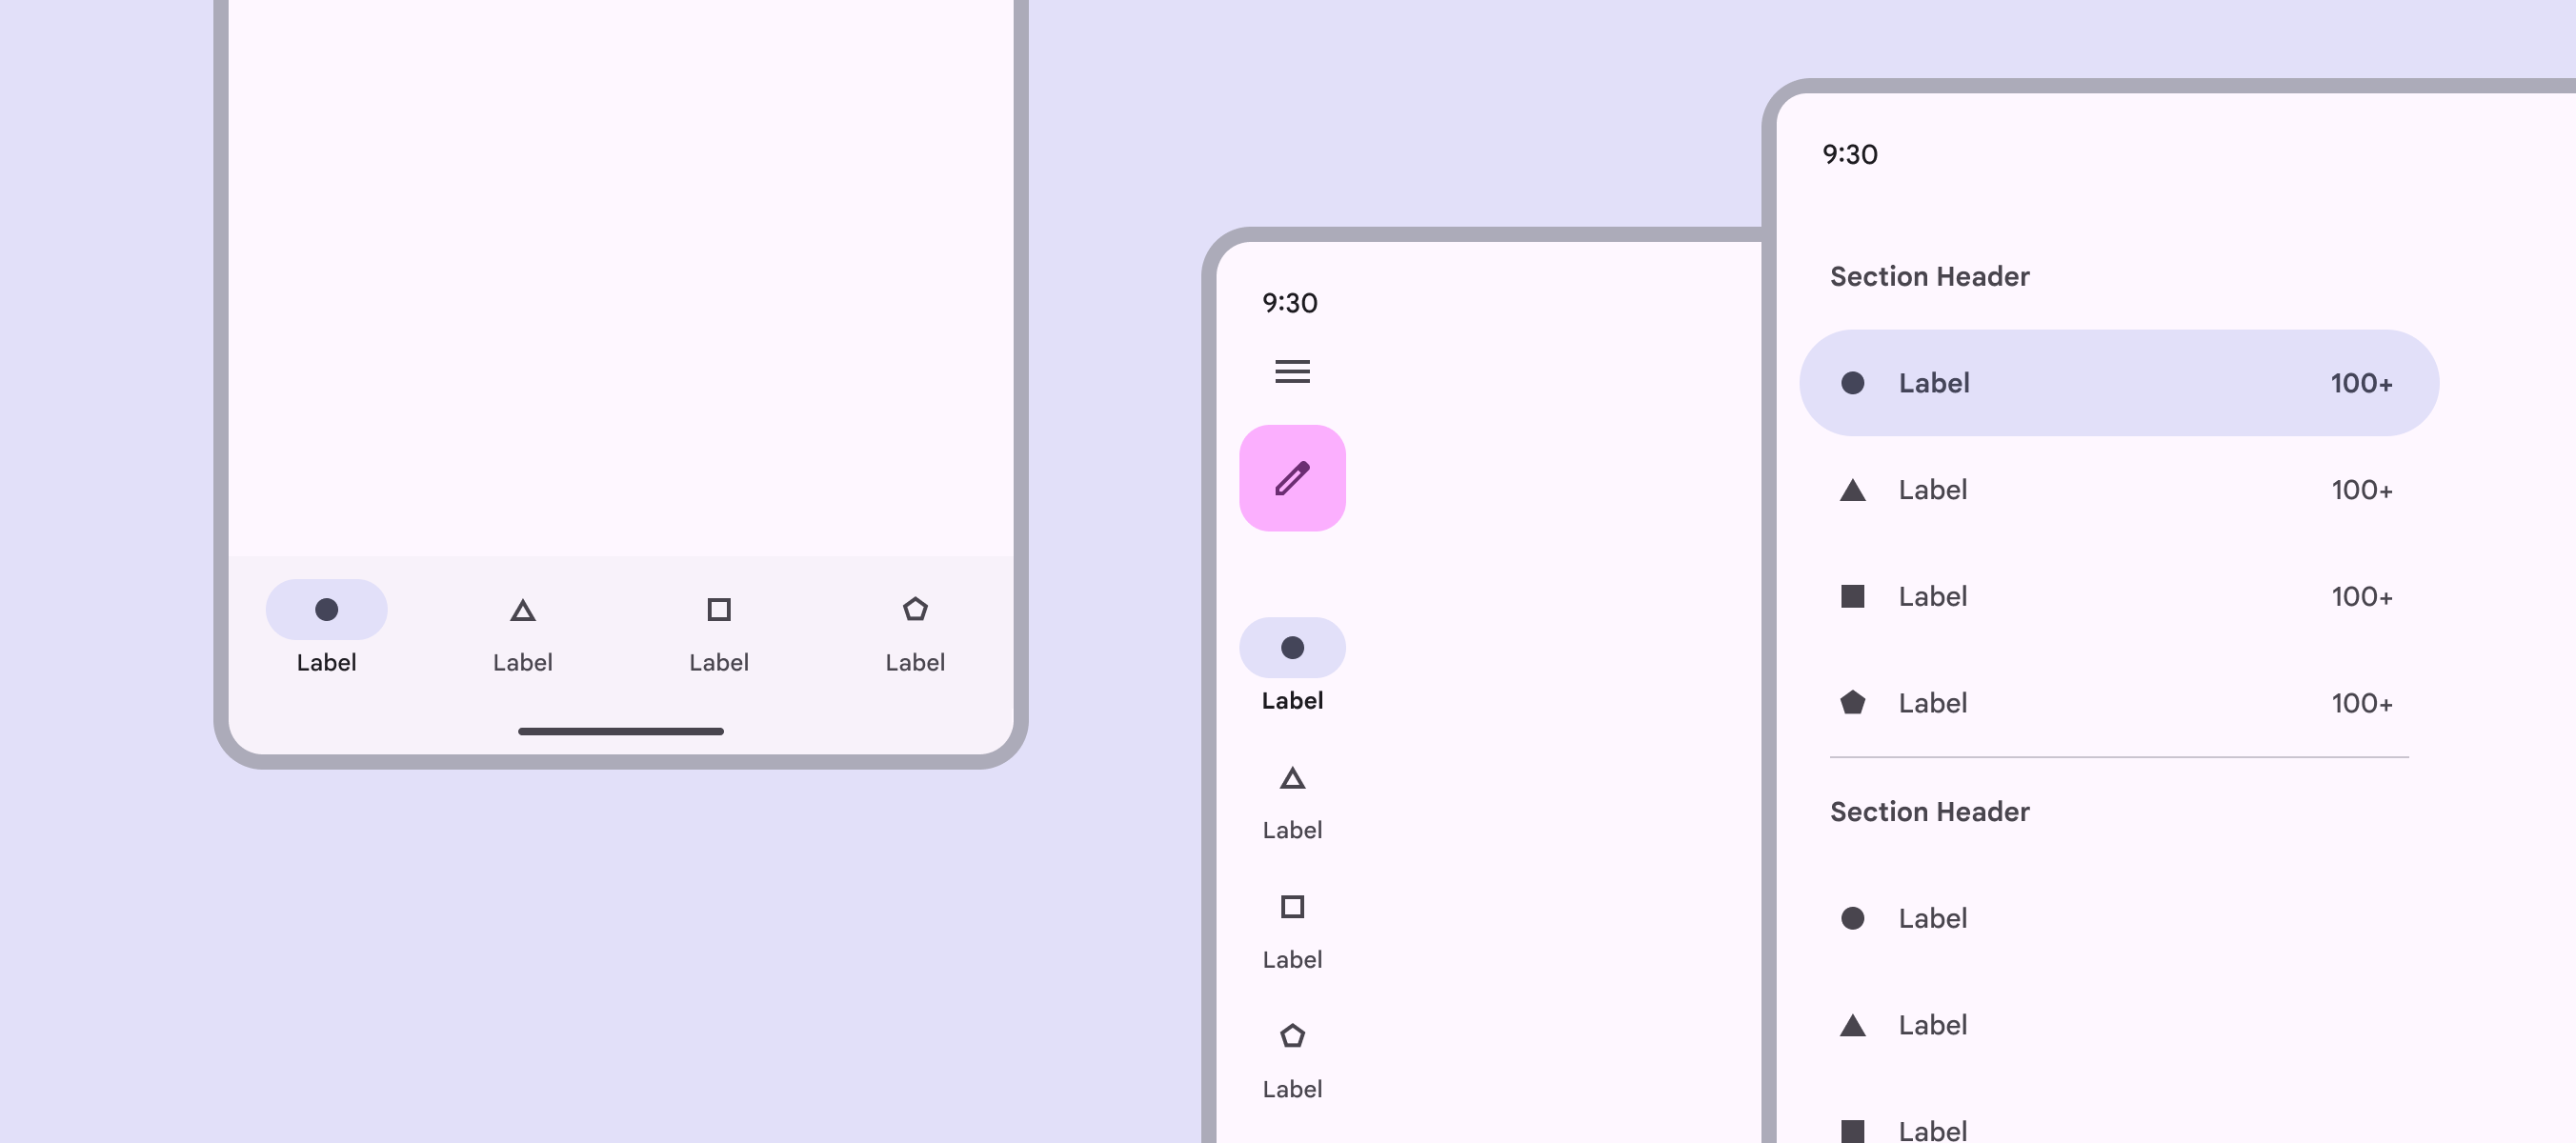
\includegraphics[width=\textwidth]{images/navigation1.png}
  \caption{Navigační prvky - převzato z \cite{layout-m3}}
  \label{pic-navigation}
\end{figure}

\subsection{Zajímavosti při tvorbě práce}
Představa a samotná tvorba práce místy přinesou nečekané komplikace, které je nutné řešit nebo redefinovat požadavek. I v tomto projektu jsem se s touto výzvou setkal.

\begin{itemize}
  \item \textbf{Problém s výběrem SQLite balíčku} nastal hned ze začátku programování aplikace. Při postupování podle dokumentace \cite{flutter-docs}, která ukazuje práci s balíčkem sqflite, jsem při čtení dokumentace balíčku zjistil, že balíček podporuje pouze Android, iOS a macOS. Vzhledem k zamýšlenému provozu i na jiných platformách bylo nutné najít alternativu. Objevený balíček Drift naštěstí podporuje všechny platformy. Navíc přinesl i bonus v kvalitní API pro dotazování nad databází bez použití jazyka SQL.
  \item Nedodělané všechny komponenty Material designu.
  \item Smazání kategorie a co transakce v ní
\end{itemize}

\section{Uživatelská příručka}
Aplikaci Budget Buddy pro správu financí lze nainstalovat na operační systém Android a Windows se zárukou bezproblémové funkčnosti podle návodu. Na operační systémy macOS a Linux je nutné aplikaci pro tyto systémy sestavit a nainstalovat (tento postup je ponechán na zdatném uživateli). Návod se týka jen vybraných platforem z důvodu testování. 

\subsection{První spuštění}
Při spuštění se zobrazí rovnou úvodní obrazovka \textit{dashboard}. Není nutné se přihlašovat, aplikace je nyní určena pouze pro jednoho uživatele a běží lokálně. Pro první spuštění jsou vložené základní kategorie transakcí a nejběžnější měny (obojí je možno upravit). 

\subsection{Úvodní obrazovka}
Úvodní obrazovka, anglicky dashboard je centrem dění pro uživatele. Poskytuje základní přehled o finanční situaci. Konkrétně zobrazuje graf kategorií, stav účtu, dnešní útratu a posledních pět transakcí. Na zařízení s větší obrazovkou je rozšířena o legendu grafu a další zajímavé číselné údaje o stavu účtu. Úvodní obrazovka není uživatelsky přizpůsobitelná.

\subsection{Přidání transakce}
Transakce se přidává tlačítkem označeným ikonou plus (na větším zařízení i doplňujícím popiskem). Na menším zařízení se tlačítko nachází v pravé dolní části obrazovky nad navigační lištou. Na větším zařízení je umístěno před prvním prvkem v navigační liště na pravé straně obrazovky. Po stistknutí se objeví dialogové okno, kde uživatel může vybrat z následujících možností:
\begin{itemize}
  \item 
\end{itemize}

\subsection{Zobrazení a úprava transakcí}
Transakce a jejich úprava se provádí na druhé obrazovce s názvem \textit{Transactions}. Výpis je proveden v seznamu, kde je přímo vidět kategorie, měna, částka, typ, datum a případná poznámka. Po kliknutí na transakci se objeví dialogové okno a je možné všechny parametry transakce upravit, případně transakci odstranit. Transakce je možné filtrovat dvěma způsoby. Můžeme nechat zobrazit jen transakce ve specifickém období (den, týden, měsíc, rok či libovolný rozsah), k čemuž slouží porstřední tlačítko v horní části. Šipky na stranách umožňují přesouvat se o zvolené období dozadu či dopředu. Dále můžeme vybírat ze všech parametrů, které jsou transakci přiřezené (kategorie, měna, typ atd.). Obrazovka s výběrem filtrů se otevře při stisknutí tlačítka \textit{Filter} s ikonou trychtýře. Při použití více filtrů se transakce zobrazí ve výpisu pokud splňuje alespoň jednu podmínku. Aktivní filtry znázorňuje červený odznak u tlačítka filtrace.

\subsection{Využití reportů}
Grafy a důležité číselné údaje se nachází na obrazovce \textit{Reports}. Je zde na výběr z pěti přednastavených možností. Které údaje chce uživatel vidět se dá nastavit tlačítkem \textit{Manage reports} pod posledním reportem. Na výběr je těchto pěti možností:
\begin{itemize}
  \item \textbf{Most spent categories} -- zobrazí sloupcový graf s pěti kategoriemi, ve~kterých je největší útrata ve~zvoleném období.
  \item \textbf{Spent during time} -- zobrazí plošný graf s vývojem útraty v~průběhu daného období. Graf je interaktivní a při najetí pohbyu kurzorem v~grafu se zobrazí hodnota pro konkrétní datum.
  \item \textbf{Interesting numbers} -- zobrazí tři buňky se zajímavými hodnotami ze zvoleného období. Konkrétně se jedná o: procento ušetřených peněz z přijmu, průměrnou denní útratu a procento transakcí v~jiné měně než českých korunách. Podle velikosti zařízení jsou buňky řazeny ve sloupci nebo řádku.
  \item \textbf{Category ratio} -- zobrazí dvě buňky s kruhovými grafy. První zobrazuje poměr kategorií v příjmech a druhý poměr kategorií ve~výdajích. Při použití na největším zařízení se zobrazí interaktivní legenda.
  \item \textbf{Income / Outcome numbers} -- zobrazí tři buňky s číselnými údaji. Kokrétně se jedná o: součet všech příjmů, součet všech výdajů a celkový stav účtu. Podle velikosti zařízení jsou buňky řazeny ve sloupci nebo řádku.
\end{itemize}

\subsection{Nastavení aplikace}
Poslední obrazovkou dostupnou z navigační lišty je nastavení (záložka \textit{Settings}). Umožňuje nastavit jak prostředí po stránce funkcí, tak i po stránce vzhledu.

\subsubsection{Úpráva kategorií}
Přidávat, mazat i upravovat kategorie je možné v záložce \textit{Categories editor}. Otevře se nová obrazovka s výpisem všech kategorií formou karet. U každé karty je znázorněna ikona, název a barva. Ikonka tužky otevře dialogové okno s možností úpravit nastavení dané kategorie (změny je nutné uložit tlačítkem \textit{Save}). Ikona popelnice po potvrzení v dialogovém okně nevratně smaže danou kategorii i ji náležící transakce. Plovoucím tlačítkem s ikonou plus se vytváří nová kategorie s uživatelem definovaný parametry.

\subsubsection{Přizpůsobení měn}
Po kliknutí na kartu \textit{Currency settings} se rozbalí seznam všech měn (název a zkratka).

\subsubsection{Přizpůsobení vzhledu}
Vzhled je možno přizpůsobit rozbalením karty \textit{Color theme}. Na výběr je ze sedmi barev, které jsou pojmenované i s náhledem konkrétního odstínu. Konkrétní barvy reprezentují jednotlivá barevná témata. Výběr tohoto tématu změní celý nádech aplikace od výrazných barev až po jemné barvy v pozadí.

\subsection{Export dat}


\section{Možná rozšíření aplikace}
Osobně si myslím, že nikdy se nedá o softwaru prohlásit, že by nepotřeboval vývoj a není možné mu dodat vylepšení. Už jen vzhledem k vnějšímu vývoji technologií a proměně uživatelských požadavků je nutné aplikaci udržovat aktuální. Se změnou požadavků se pojí rozšíření o nové funkce a nebo naopak odstranění funkcí nepoužívaných.

\begin{enumerate}
  \item Možnost založit více účtů
  \item Umožnit nastavení vlastní měny
  \item Import dat z jiných aplikací
  \item Vylepšení uživatelského rozhraní
\end{enumerate}

\begin{kiconclusions}
Tady bude závěr.
\end{kiconclusions}

\begin{kiconclusions}[english]
Here will be conclusion.
\end{kiconclusions}

% ----- tady začíná to co v práci bylo dáno

%%%  Po přeložení programem CSLaTeX (třikrát) je potřeba použít
%%%  program DVIPS a takto získaný PostScriptový soubor vytisknout
%%%  na PostScriptové tiskárně nebo pomocí programu GhostScript.
%%%
%%%  Rovněž je možné použít program DVIPDFM a vytvořit z dokumentu
%%%  soubor ve formátu PDF včetně hypertextových odkazů.

%%% Argument `joinlists' způsobí zřetězení seznamů obrázků, tabulek,
%%% vět a zdrojových kódů. Není-li použít, všechny seznamy jsou
%%% uvedeny na samostatných stránkách.

%%  'encoding=kódování' pro kódování tohoto a vložených zdrojových
%%  textů v kódování jiném než výchozím utf8

%% -------------------------------------------------------------------

%% Sazba povinné bibliografie, za přílohami (případně i za seznamem
%% zkratek). Při použití BibLaTeXu použijte makro
%% \printbibliography. jinak prostředí thebibliography. Ne obojí!

%% Sazba i v textu necitovaných zdrojů, při použití
%% BibLaTeXu. Volitelné.
%% \nocite{*}
%% Vlastní sazba bibliografie při použití BibLaTeXu.

\printbibliography
\nocite{*}


%% Sazba volitelného rejstříku, za bibliografií.
%% \printindex
%% \printglossaries
\end{document}
